\documentclass[a4paper,12pt]{article}
\renewcommand{\baselinestretch}{1.5} 
\usepackage[utf8]{inputenc}
\usepackage[acronym,toc]{glossaries}
\usepackage{url}
\usepackage{booktabs}
\usepackage{appendix}
\usepackage{setspace} % for \onehalfspacing and \singlespacing macros
%\singlespacing
\usepackage{etoolbox}
\AtBeginEnvironment{quote}{\singlespacing\small}

%Necessary packages
\usepackage[english]{babel}
\usepackage{amsmath, amsthm, amssymb}
\usepackage{a4wide}
\usepackage{verbatim}
\usepackage{import}
%\usepackage{xparse}
\usepackage{enumerate}

%graphical packages
\usepackage{csvsimple}
\usepackage{float}
\usepackage{algorithm2e}
\usepackage{sidecap}
\usepackage{wrapfig}
\usepackage[final]{graphicx}
\usepackage[space]{grffile}
\usepackage{caption}
\usepackage{subcaption}
\usepackage[section]{placeins}
\usepackage{tikz}
\usepackage{color}
\usepackage{eurosym}
\usepackage{rotating}
\usepackage{amstext} % for \text
\usepackage{natbib}
\usepackage{hyperref}
\hypersetup{final}
\hypersetup{
    colorlinks=true,
    linkcolor=cyan,
    filecolor=cyan,      
    urlcolor=cyan,
    citecolor=cyan
}

%Indentation
\setlength\parindent{20pt}
%Theorems, Definition, ordered by section
\theoremstyle{plain}
\newtheorem{theorem}{Theorem}[section]
\theoremstyle{definition}
\newtheorem{definition}[theorem]{Definition}
\theoremstyle{definition}
\newtheorem{lemma}[theorem]{Lemma}
\theoremstyle{definition}
\newtheorem{proposition}[theorem]{Proposition}
\theoremstyle{definition}
\newtheorem{corollary}[theorem]{Corollary}



%%%%% Title %%%%%
\title{Agricultural child labour in response to climate change\footnote{Acknowledgement goes here.}}
\author{Mathias Weidinger\footnote{Maastricht University and UNU-MERIT, \href{mailto:m.weidinger@maastrichtuniversit.nl}{\texttt{m.weidinger@maastrichtuniversity.nl}}}}
\date{\today \footnote{The latest version of this paper is available at \href{https://www.mathiasweidinger.com}{\texttt{mathiasweidinger.com}}} \\ First version: November 2020}

\begin{document}

\maketitle

\begin{abstract}
Anthropogenic climate change severely impacts agriculture in developing countries and with it the millions of children actively involved in that sector. Economic theory can be used to characterise the effects that climate change might have on agricultural child labour. Merging two strands of theoretical literature, from Environmental Economics and Development Economics, this paper presents a simple household decision model of child labour supply under climate change. To take the model to the data, I combine a household panel from Nigeria with geo-coded weather records and estimate the dose-response function.

% ADD some detail about the outcomes once they are available...and feed them into three models: structural estimates via maximum likelihood are compared with those obtained from a commonly used non-parametric method (B-splines) and those of the recently proposed spatial first difference estimator. 
\end{abstract}
% J22=Time allocation and labour supply
% J43=Agricultural Labour Markets
% I32=Measurement and Analysis of Poverty
% Q54=Climate, Natural Disasters, Global Warming
% D11=Consumer Economics: Theory
% D12=Consumer Economics Empirical Analysis
% D13 Household Production and intrahousehold allocation

\textit{JEL}: D11, D12, D13, J22, J43, I32, Q54

\textit{Keywords}: child labour, climate, agriculture, global warming

\clearpage



%chapters:

\section{Introduction}
\label{intro}

Globally, nearly one in ten children are subjected to child labour and the fraction is twice as high in Africa. On any given day in 2016, 152 million children aged 5-17 were in some form of child labour; half of them worked under hazardous conditions \citep{ILO2017}. The consequences of this are well-understood:

\begin{quote}
    Child labour can result in extreme bodily and mental harm, and even death. It can lead to slavery and sexual or economic exploitation. And in nearly every case, it cuts children off from schooling and health care, restricting their fundamental rights and threatening their futures \citep{UNICEF2020}.\footnote{For a recent review of the adverse health outcomes of child labour, see \citet{Ibrahim2018}.}
\end{quote}

Unfortunately, Child labour is notoriously difficult to regulate. This is in part due to its informality: Most child labour is unpaid and takes place far off the formal labour market, on family farms or in family owned enterprises. Consequently, the compliance costs of anti child labour legislation are so high that even where such laws are in place, enforcement tends to be lax or, all too often, entirely absent.\footnote{Note that this is not necessarily due to negligence by the government. Most countries with high rates of child labour also suffer from limited fiscal capacity and, consequently, prohibitively small budgets.} Despite sustained international efforts to eliminate it, child labour decreased by only one percent in 2008-2012 and the \citet{ILO2017} estimates that at the current rate of progress, 121 million children will still be working in 2025.\footnote{The International Convention on the Rights of the Child (ICRC) recognises the right of every child to be protected from economic exploitation and from performing work that is hazardous or harmful to their health and development or that interferes with their education. The ILO conventions on minimum age for admission to employment (no. 138, ratified by 173 countries) and on the the elimination of the worst forms of child labour (no. 182, ratified by 187 countries) are binding international agreements to this effect. Targets 8.7 and 16.2 of the United Nation's Sustainable Development Goals additionally target child labour, pledging to end it in all its forms by 2025.}

Disaggregating the data reveals that 59 per cent of working children in Africa are between 5 and 11 years old and that almost nine in ten of them work in agriculture - 61.4 million children in absolute terms. The uniquely high concentration of child labour in agriculture - particularly in Sub-Saharan Africa (SSA) - begs a question: What happens to these children if agriculture becomes an increasingly unstable sector? Do they work more or less hours on average? Does their work become more or less hazardous? How is their overall welfare affected? These concerns bear unprecedented relevance in the wake of anthropogenic climate change.

There is mounting evidence that the human-induced accumulation of Green House Gases (GHG) in the earth's atmosphere has caused the global climate to change and will continue to do so in the coming centuries \citep{Pachauri2014}. Many new record highs suggest that the earth's mean temperature is increasing. \citet{Munasinghe2012}, for instance, show that the frequency of extremely high temperatures across the global landmass increased tenfold between the beginning of the twentieth century and 1999–2008. The high frequency of new record lows over the same period suggests a simultaneous rise in the variance of temperature \citep{Auffhammer2014a}. As a consequence, climate change persistently increases the probabilities of extreme weather events such as droughts, floods, snow storms, heat waves, cyclones, and hurricanes \citep{Pachauri2014}. These changes in the natural environment profoundly alter the setting for human economic activity on planet earth.

It is of course true that climate change affects different regions in different ways. This heterogeneity has inspired some to speculate, whether the negative impacts experienced in some areas could be offset by positive effects elsewhere\footnote{For instance, while agricultural yields are likely to decrease in SSA, some conjecture that large parts of northern Eurasia, which are currently covered by permafrost, could become arable as temperatures rise. Moreover, an elevated concentration of atmospheric CO$_2$ reduces water stress in plants and may make them grow faster. This phenomenon, known as CO$_2$-stimulation, and its beneficial effect on crop yields remain understudied and, therefore, unincorporated in most projections \citep[e.g., in][]{Schlenker2010}.}, or be it in strictly economic terms. \citet{Tol2009}, for instance, notes that ``although the world population is concentrated in the tropics, where the initial effects of climate change are probably negative, the relatively smaller size of the economy in these areas means that gains for the high-income areas of the world exceed losses in the low-income areas''. He later qualifies this statement, adding that, in the long term, warming above 1-2 degrees will likely have negative total effects. But even for the short-term, arguments like Tol's ought to be read with some scepticism. They are not inherently incorrect, but their accounting method entirely ignores the distributional consequences of climate change (and indirect economic effects that stem from them).

The world's richest countries, which are predominantly situated in  the global north, are responsible for almost eighty percent\footnote{The percentage is even higher when accounting for final consumption of goods, since great part of GHG emissions in low and middle income countries stem from the production of export goods, predominantly destined for high income countries.} of GHG emissions in 1850-2011 and high income countries continue to emit the most GHGs by far\footnote{Note, however, that in terms relative to 1990 most high income countries now have lower annual growth rate of emissions whereas lower and middle income countries have increased their emissions substantially.} \citep{Ritchie2017}. Due to their location, high income countries also experience more benign effects of climate change compared to their more vulnerable counterparts further south, which face the harshest consequences. Intensified temperature extremes, precipitation anomalies, and natural disasters are all projected to disproportionately afflict Latin America, South Asia and the Pacific, and Sub-Saharan Africa. Together, their populations account for the vast majority of human kind. Thus, Climate Change exacerbates existing global inequalities and there is an argument to be made for distributional considerations beyond simple aggregate cost-benefit analysis. Distributional aspects are highly relevant for migration policy, International cooperation, and conflict-prevention efforts - not to mention global solidarity.

In SSA alone, the effects of climate change are responsible for at least 1,000 deaths, 13 million people seriously afflicted\footnote{This includes individuals who were injured, left homeless, food insecure, or lacking water and sanitation.}, and 520 USD million in direct economic damages since 2000. One-third of the world’s droughts occur in SSA, and the frequency of storms and floods is growing fastest in this region \citep{IMF2020}. Agricultural yields, meanwhile, are projected to fall significantly for the continent's four most important food crops: by 22 percent for maize, 17 percent for Sorghum, Millet and Groundnut, and eight percent for cassava \citep{Schlenker2010}. Similar negative impacts have been projected for major cash-crops like coffee \citep{Craparo2015}\footnote{For contrasting findings, based on CO$_2$-stimulation effects, see \citep{DaMatta2019}.} or cocoa \citep{Boeckx2020}. These findings place agriculture at the centre of climate vulnerability, and with it the millions of children working on farms throughout the world.

Even so, there is virtually no literature investigating the implications of these negative effects for child labour. The little empirical evidence there is displays three common flaws: limited data, misspecification, and a lack of theoretical underpinning. These shortcomings and the policy-relevance and urgency\footnote{Given the proximity of the 2025 deadline scoped by SDG 8.} of the child labour debate provide a clear motivation for further research. To narrow the gap, this paper is dedicated to analysing the effects of climate change on the prevalence of child labour in agriculture, as well as their implications for household and children’s welfare.

This paper is organised as follows. Following a detailed overview of the literature in section~\ref{sec:literature}, section~\ref{sec:model} extends the economic theory of child labour to account for a sustained shock to household production due to climate change. The resulting model produces theoretically sound hypotheses that can be tested empirically. Section~\ref{sec:empirical_analysis} outlines the empirical problem and introduces an econometric framework to tackle it. The methods used mend the shortcomings noted in the literature; a longitudinal data set from Nigeria (2010-2019) is combined with geocoded weather data from suitable ground level stations, supplemented by satellite-based estimates. The findings drawn from this analysis are discussed in section~\ref{sec:findings}. %In section~\ref{sec:simulation}, I perform a structural estimation of the model developed in chapter two. Once calibrated to the data, the effects of future climate change are simulated using the predictions of a global climate model (GCM) instead of historical weather data. The results offer novel and relevant input for weighing the costs and benefits of GHG emission abatement – not only monetarily but through the lens of child welfare.
Section~\ref{sec:conclusion} identifies actionable policies and concludes.

\section{Literature}
\label{sec:literature}
The topic at hand lies at the intersection of various strands of literature: Development and Labour Economics have provided some models of Child labour. Environmental and Resource Economics feature a relatively recent and fast-growing literature on the economic effects of climate change. Lastly, Agronomy has long studied the effects of weather shocks on agricultural output. This section offers an overview of the first and the second of these fields, subsuming the third within the more recent climate studies, which draw heavily from it.

\subsection{Child Labour}
\label{sub:child_labour}
Child labour appears early as a topic in the economics literature. Among those who discussed its prevalence in Europe during the Industrial Revolution were Smith, Malthus, and Marx.\footnote{With the exception of Malthus, the early economists viewed children as investment goods. Marx, in particular, remarked that ``all family ties among the proletarians are torn asunder, and their children transformed into simple articles of commerce and instruments of labour'' \citep{Marx1848}.} About a century later, the inception of human capital theory \citep{Mincer1958, Schultz1961, Becker1964} fundamentally transformed the research agenda in labour economics and, as a corollary, gave some impetus to the study of child labour \citep[see e.g.][]{Rosenzweig1977}. The seminal contribution by \citet{Basu1998} eventually launched an enduring proliferation of the literature on child labour \citep{Edmonds2007} in both  theoretical and applied economics.\footnote{for a recent overview, see the dedicated volume by \citet{Posso2020}.}

Child labour is commonly modelled as a product of a constrained optimization exercise, undertaken as if each household were one collective decision maker. In practice, this implies that benevolent\footnote{On the credibility and extent of such benevolence and its implications, see \citet{Bhalotra2002}.} household heads take decisions for the entire household in a nearly utilitarian fashion.\footnote{Nearly because child leisure is strictly preferred to child work and it is unclear how this preference affects the household's aggregate utility.} \citet{Basu1998} proved so influential because they formalized two long-held conjectures in axioms that became the bedrock of child labour theory.

The first of them, termed the `luxury axiom', characterises parents' preferences over child labour as lexicographic: child labour occurs if and only if families cannot cover their subsistence needs without it.\footnote{This axiom obtains its name from that fact that, from the household's perspective, child leisure is a luxury good, more of which is consumed as income rises. An early proponent of this inverse relationship, Thomas Malthus noted that the prevalence of child labour in the late 18th century was proof that families were unable to meet their most basic needs \citep[see][]{Edmonds2007}.} This characterization of preferences would imply a strictly negative relationship between household income and the amount of child labour supplied by a household - a testable hypothesis for which \citet{Basu1998} have drawn substantial criticism \citep[see e.g.][]{Edmonds2012}. Most notably, \citet{Bhalotra2000,Bhalotra2003} observe that children of land-rich families are often more likely to be in work than those of land-poor households.

Subsequent replications of this observation spurred numerous attempts at solving the `wealth paradox' that had become apparent in child labour theory. \citet{Bhalotra2003} attribute their findings to imperfections in the labour and credit markets as well as household size: If labour markets are imperfect, child labour is increasing in farm size and decreasing in household size, while access to credit spreads the effects out over time (viz., consumption smoothing). Others attempt to resolve the paradox by altering the original luxury axiom. \citet{Basu2010}, for instance, propose that the relationship between land wealth and child labour is not monotone - positive or negative - but follows an inverted U-shape. Therefore, child labour will eventually decrease as households become wealthier. Initially, however, an increase in land wealth increases both income and the marginal benefit from child labour. It is only after a structural threshold, beyond which child labour's marginal cost outweighs its benefits, that the relationship reverses direction and child labour decreases for good. This threshold could, for instance, be the income at which the household can afford to contract external labour. \footnote{Note that this narrative - things need to worsen before they can get better -  resembles the well-known tale of growth and inequality described by the Kuznets Curve \citep{Kuznets1955, Kuznets1963} and that of growth and pollution described by the Environmental Kuznets Curve (EKC). Notwithstanding their popularity, these narratives remain empirically unsubstantiated. See, however, \citet{Piketty2014} for evidence against the Kuznets curve, and \citet{Mills2009} and \citet{Ozokcu2017} for similar results regarding the EKC.} 

\citet{Dwibedi2017} propose another version of the luxury axiom by which child labour decreases in \textit{relative} poverty. This allows for child labour to rise even as every household is made wealthier, as long as the relative distance in wealth between them increases. Their observation that pareto-dominance may not fully characterise poverty mirrors an ongoing debate.\footnote{For poverty measurement techniques of both absolute and relative poverty, as well as their distinction, see \citet{Sen1976} and \citet{Ravallion2020}.} Absolute measures of poverty are prone to underestimation and run risk to ignore the amplification of human misery that springs from inequality. Relative poverty indicators, on the other hand, are only strictly relevant in conjunction with absolute measures - a millionaire surrounded by billionaires is not `poor' in the common sense of the word.\footnote{This is assuming that the currency used is not a highly inflated one (e.g. Euros rather than Venezuelan Bolívars) and that price levels are comparable to those in the real world.} While hybrid measures, like `weakly relative poverty' \citep{Ravallion2009} exist, I am not aware of attempts to characterise child labour responses to varying degrees of absolute poverty and income inequality in an integrated framework.\footnote{\citet{DAlessandro2016} show how political support for child labour regulation is shaped by inequality as it affects the welfare of low skilled adults differently than that of highly skilled ones.} Contested to this day, the wealth paradox and the luxury axiom continue to inspire this type of research.\footnote{For more examples see e.g. \citet{Dumas2007}, \citet{DelCarpio2008}, \citet{DelCarpio2012}, \citet{Edmonds2012}, \citet{Sarkar2016}, \citet{Oryoie2017}, and \citet{Noack2019}.}

As for their second premise, \citet{Basu1998} model child labour as a substitute for adult labour from the firm's perspective - a notion captured in their `substitution axiom'. The degree of such substitutability has been debated as well. Due to their lack in experience and bodily development, children are commonly thought to be less suited for most jobs in terms of their productive potential. \citet{Bar2009} model children to be productive (to some degree) only under adult supervision and entirely unproductive otherwise. While it extends the theory beyond the substitution axiom, their model is likely too restrictive. Toddlers aside, children - including those of very young ages - are capable of performing many simple tasks, making them productive labourers in their own right. This considered, the model presented in section~\ref{sec:model} allows for a more realistic characterisation of substitution with and without supervision.

As the literature continues to append Basu and Van's model, it also outgrows it. Many of the more recent studies pay less attention to resolving the wealth paradox or characterising substitution between adult and child labour, but explore instead how child labour is affected through other channels. A natural extension is to explicitly model the allocation of children's time between work and education in terms of opportunity cost. Dynamic models, owing much to human capital theory, describe how households weigh the immediate short term benefits of income-generating child labour against  children's future earning ability that increases in education \citep[see e.g.][]{Bar2009,Pal2012,Dendir2014, Edmonds2014,Chakraborty2018}. This crucially depends on the current extent of deprivation, on the rate by which parents discount the future, on whether they view their children's future earnings as a consumption smoothing mechanism for themselves (e.g. during old age), and also on their altruism towards their children.\footnote{Knowing that they may well die before the fruits of child education can be reaped, purely self-interested parents may prefer sending their children to work and enjoy additional income presently.}

Another extension is to model the role of markets. \citet{Baland2000},\citet{Bhalotra2003}, and \citet{Dumas2007}  investigate how imperfections in the credit and (adult-)labour markets could cause households to deploy relatively more or less child labour. \citet{Basu2010} rely, in part, on the absence of functioning labour markets to arrive at their inverted U-shape. \citet{Dumas2013,Dumas2015,Dumas2020} characterises a whole range of scenarios by selectively switching markets on and off one at a time and observing the effect on child labour in her model. To date, the literature largely confirms the moderating effects of labour markets and, less clearly so, the deferring effects of credit markets. Overall, child labour theory has evolved into a framework, capable of analysing child labour in relation to the wider micro-economic context that surrounds it.

Finally, the studies that are closest related to mine focus on the effects of external shocks on such a system. \citet{Dumas2015,Dumas2020} uses rainfall as a shock on household production in agriculture and, thus, indirectly on the households' child labour supply decision. She finds that, in the case of Tanzania, child labour increases in rainfall and that this increase is attenuated if the household has access to a well-functioning labour market. Moreover, her findings indicate that credit markets are less effective in smoothing such rainfall shocks. Manual labour provision can solve the household's problem contemporaneously (harvesting or sowing before the crops rot or the ground dries up), whereas consumption smoothing by credit only protracts costs into the future as long as the underlying problem remains unsolved. Of course, access to credit is usually quite limited in developing countries and particularly so among the poorest. Furthermore, there is only so much credit a poor farming household can take up, assuming there is a functioning market, before it is worse off than before. Lastly, climate change is neither idiosyncratic nor transient, which makes it virtually impossible to insure against.  

\citet{Boutin2014} is the only paper to date which explicitly studies the link between climate change and child labour. Boutin's approach is, however, less direct than that used in \citeauthor{Dumas2020}' rain-shock study. She measures climate vulnerability rather than effectuated climate change itself. Her independent variable is an aggregate of two indices that ``take into account the multidimensionality of climate change"; one index on biophysical vulnerability defined over climate volatility, variability, landscape typology and soil structure, and another index measuring a community's adaptive capacities, which takes into account diversification strategies, financial capacities, and community-level amenities. One advantage of using such a composite index is that it overcomes potential endogeneity problems:

\begin{quote}
Households whose income and assets are most vulnerable to climate damage will benefit more from income diversification generated by child labour than other households. Consequently, they might be more likely to have a child working that can smooth consumption in the event of a severe climate shock. This would also be the case if risk-adverse households are more likely to have working children in order to diversify income sources and are also more likely to invest in self-protection mechanisms \citep[][p.5]{Boutin2014}.
\end{quote}

Endogeneity of this kind aside, concerns about measurement error as well as the cross-sectional nature of Boutin's data still complicate causal inference. Her climate vulnerability index is certainly a valuable contribution, especially when it comes to designing forward looking adaptation policies. Much of the pertinent policy debate, however, centres around quantifying the impacts of exposures to adverse effects of climate change rather than the human response to an increase in vulnerability per se.\footnote{On the attribution of a single event to climate change, see \citet{Hansen2014}.} Therefore, this paper focuses on the effects of eventuated climate change - more frequent episodes of drought or flooding and persistent shifts in mean temperature and precipitation - on child labour. Although \citeauthor{Boutin2014}'s metrics are different from the ones deployed here (vulnerability towards climate change versus actual, exogenously apportioned exposure to its negative effects), her findings provide a benchmark against which to compare the present study. \citeauthor{Boutin2014} finds that climate vulnerability negatively affects child labour incidence and intensity, while it does not seem to have an impact on household chores. Thus, she concludes that child labour is an adjustment variable to local labour market conditions but not correlated with a given communities’ joint climate resilience \citep{Boutin2014}. 

The identification approach in this paper is much closer related to the rain induced shock used in \citet{Dumas2020}; I use multiple weather-component variables to shock the system and relate them back to changes in the climate. To guide the formulation of this second part of my model, I now offer a brief overview of the literature on climate change and its effects on the socio-economic sphere. 

\subsection{Agriculture and Labour Supply}
\label{sub:agriculture_and_labour_supply}

In the field of Agricultural, Resource and Environmental Economics (ARE) there is a long history of using weather measures as explanatory variables in statistical models of agricultural productivity \citep[e.g.][]{Fisher1925}. The reason for this is simple: Setting labour, machines, and fertilizer aside, the inputs to agricultural production are biophysical variables like soil nutrients, sunlight, rainfall, temperature, or pests. As such, a change in weather affects them much more immediately than it would affect most inputs in other sectors. But there are also considerable social and economic factors at play; Crop choice, the use of fertilizers or pesticides, capital and machinery used to till and harvest, and long-term planning of plot use rotation are all examples of human decision variables that interact with the aforementioned physical ones. The exact form of these human-nature interactions are subject to economic decision-making and depend on the farmers’ preferences as well as on their constraints, environmental and otherwise.  Figure~\ref{fig:production_auffhammer} schematically depicts such a production process from the farmer's perspective.

\begin{figure}[t!]
    \centering
    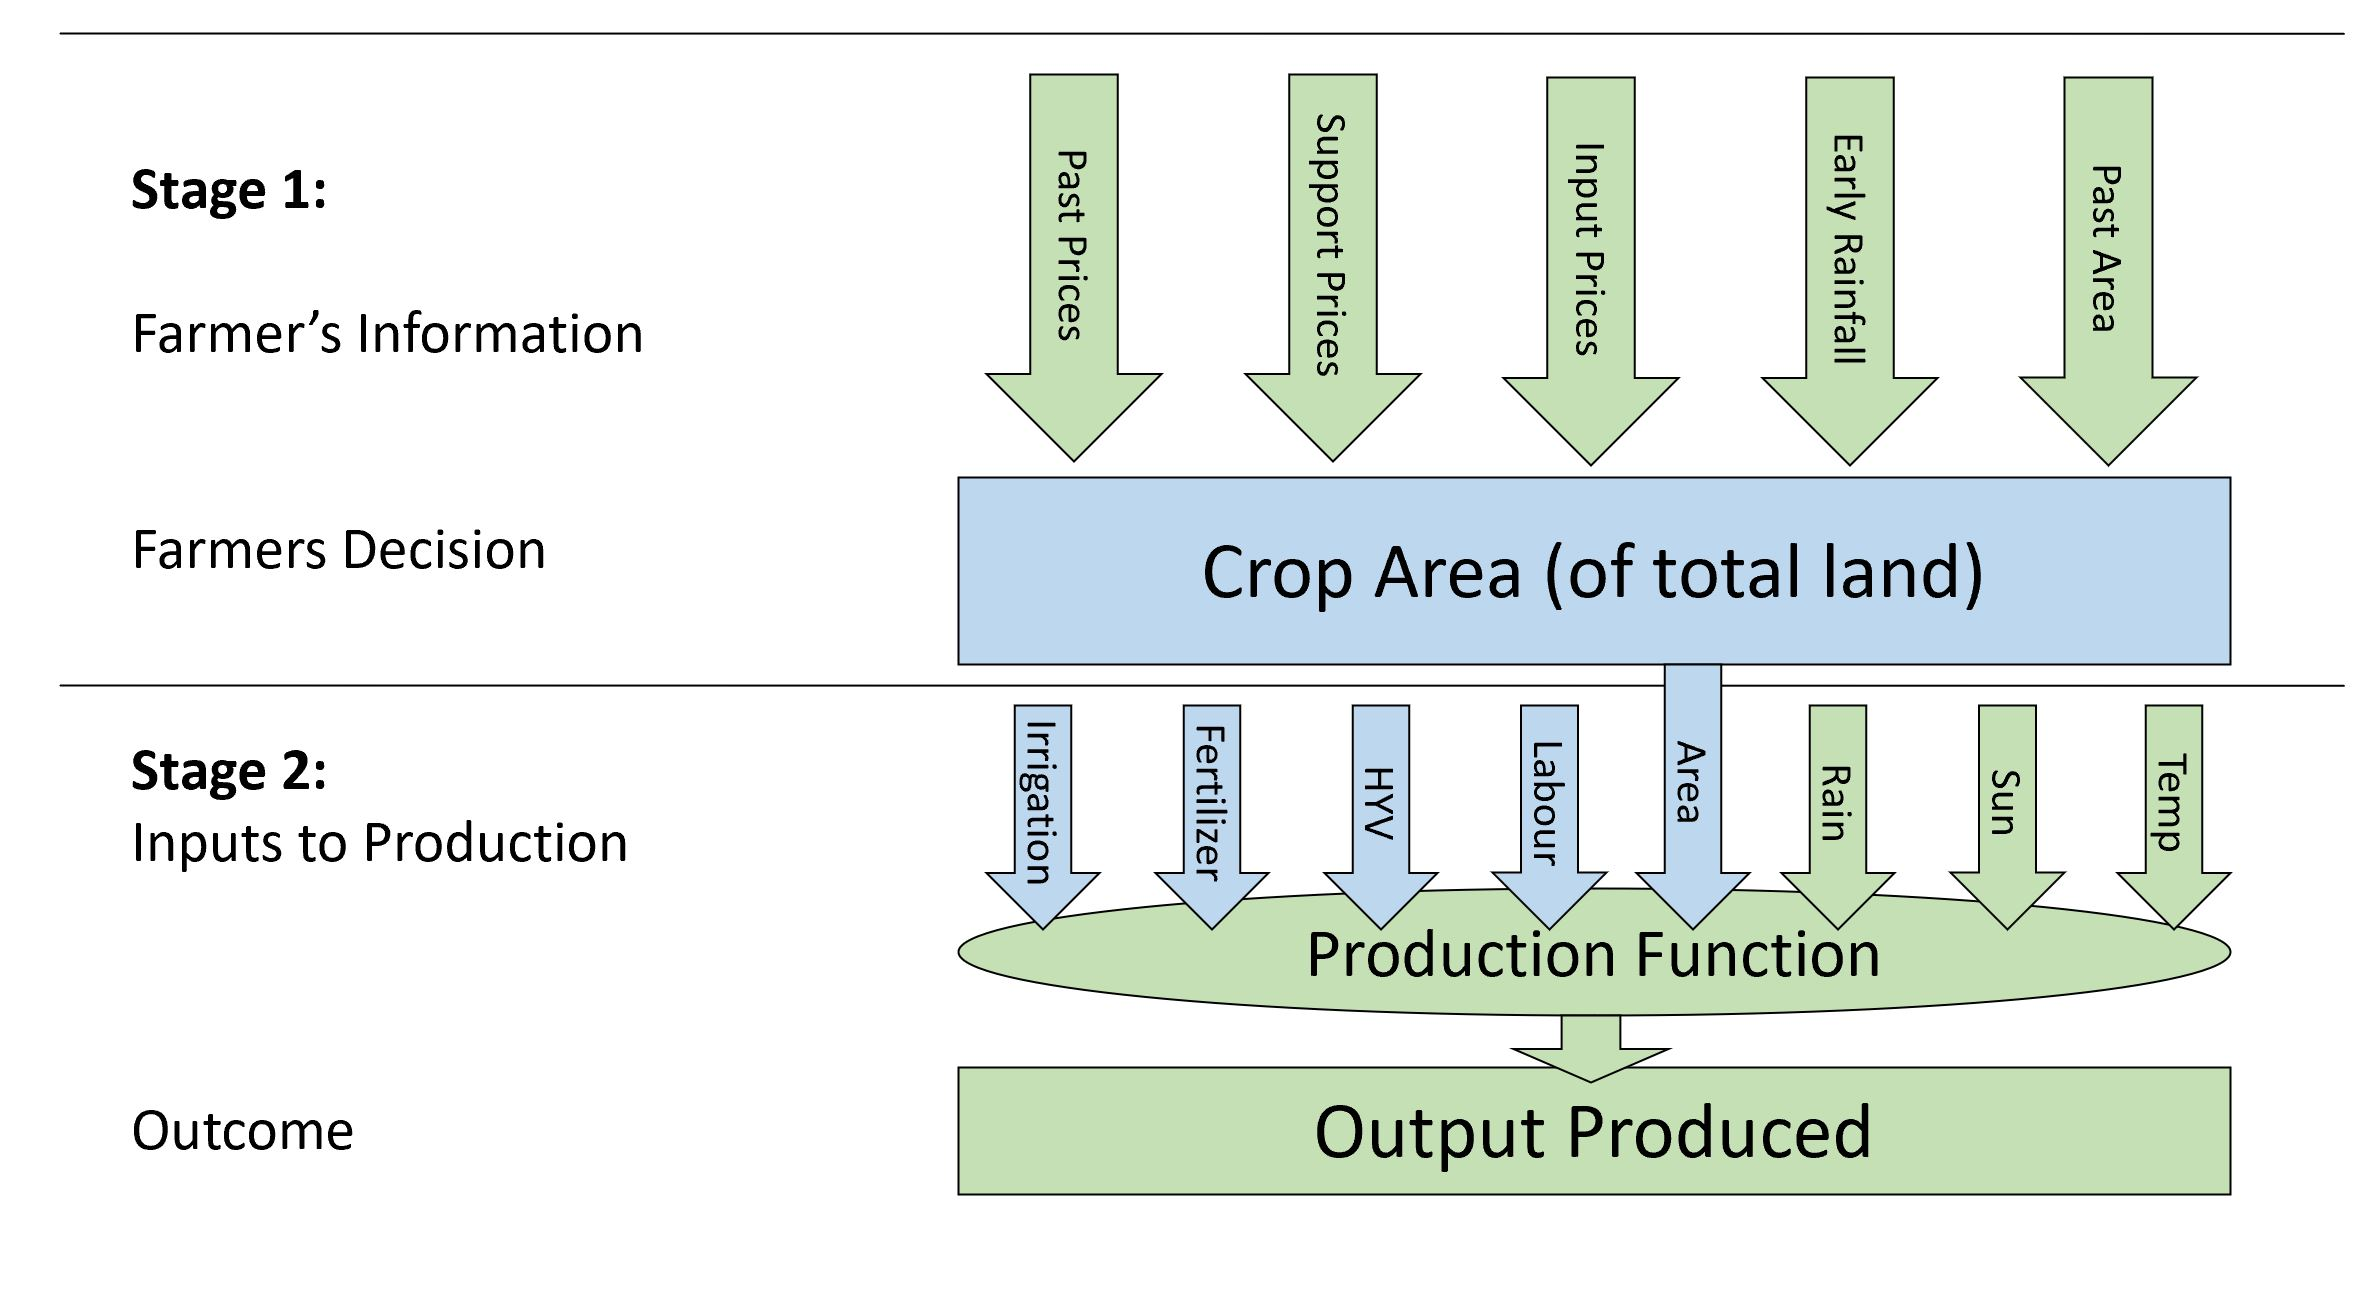
\includegraphics[scale=0.5]{fig_production_auffhammer.JPG}
    \caption{The farmer's problem.}
    \caption*{\footnotesize{\textit{Note:} At stage 1, the farmer observes relevant information, the realization of which is exogenous. Based on this, the farmer apportions some land for planting a given crop. In stage 2, inputs enter the production function (HYV = high yield variety). Inputs depicted by blue arrows are choice variables for the farmer, green ones are not. \textit{Source:} adapted from \citet{Auffhammer2014b}.}}
    \label{fig:production_auffhammer}
\end{figure}

Labour supply depends in many ways on all the other factors to fall in place first: No additional harvesters are needed if, for example, a drought wipes out your crops before they are ripe. It is this connection between the physical conditions for agriculture and the human labour inputs to it, which may prove helpful for exploring the more specific characteristics of child labour supply in that sector. 

One consequence of the complex nature-human interactions that characterise agricultural production is that the productivity of labour cannot be observed directly by the executive farmer, even if he were to monitor all workers constantly. Indirect measures of productivity, such as the number of tasks performed per worker, are also unavailable for most of the productive cycle: At harvest, one can judge the amount of produce harvested per worker and, at planting, the quantity of seeds sown or the area of land covered. Between planting and harvesting, however, labour productivity is not straight forward to measure indirectly as growth and crop quality are mostly determined by environmental factors. Since total production at the end of the harvest is a complex function of many worker's individual contributions and of the environment over time, individual workers' inputs cannot be easily disaggregated or compared. Thus an informational asymmetry arises. 

%Assuming that workers value leisure, the ex-post non-disaggregatability of total production means that they would like to freeride whenever they can knowing that the principal will be unable to detect their defecting behaviour. This moral hazard arises for all workers. For external wage labourers, the asymmetry is aggravated additionally by the fact that their wages are usually paid per week, day, or hour spent on the employing farm rather than by productivity units actually realised (remember that these are incommensurable most of the time). Avoiding work could be lucrative to the extent that there is still sufficient output at the end so that wages are paid and consumption needs are met. The employer only has one option to limit this behaviour, which is direct oversight. Overseeing labour becomes increasingly costly as farm size and labour force increase, yielding it unprofitable for most farms larger than a single plot \citep{Sen1981a}.

One result of this is the inverse relationship between a farm's size and its productivity, which was first noted in the case of India \citep{Sen1962} and has since been evidenced across the developing world. The literature shows quite convincingly that - holding inputs constant - small family owned farms are more productive than bigger enterprises. There is disagreement, however, on whether this is due to the lesser extent of moral hazard (e.g. shirking) among family members vis a vis wage workers\footnote{Household members have a direct interest in maximising farm output because their consumption is directly dependent on it. Wage workers, on the other hand, can benefit from defecting behaviour as long as output remains high enough so that a decline can credibly be attributed to solely environmental factors and wages continue to be paid.}, or due to the spatial dispersion of workers on bigger farms which drives up monitoring costs \citep{Sen1981a}. Either way, free-riding seems to be less of a problem on family-farms without labour market connections.

On the other hand, labour markets are crucial for insuring against crop failure. \citet{Kochar1999} presents evidence suggesting that the smoothness of household consumption in the presence of farm-specific crop income shocks reflects the ability of households to smooth income directly, by increasing their market hours of work. This is an early pointer to the important role that labour markets play in household consumption smoothing and, consequently, its effects on child labour allocation discussed in \citet{Dumas2015,Dumas2020}.

\subsection{Economic Effects of Climate Change}
\label{sub:economic_effects_of_climate_change}

 Since child labour is not prominently featured as a topic in the ARE, the importance of this literature for the present study lies predominantly in providing a framework that can link climate and weather to socio-economic phenomena \textit{like} child labour.

Indeed, the relatively recent empirical literature on the economic impacts of climate change has turned the spotlight onto quantifying the effect of climate on many different socio-economic outcomes. Table \ref{tab:ARE_lit} gives a non-exhaustive list of such studies. Most of them report highly nonlinear relationships between climate and the outcomes of interest \citep[e.g.][]{Schlenker2009,Burke2015}, and warm temperatures seem to be a particularly relevant factor for many climate responses \citep{Auffhammer2013}.

\begin{table}[t!]
    \singlespacing
    \centering
    \caption{Selected climate impact studies from ARE Economics.}
    \caption*{\footnotesize{\textit{Notes:} Studies by subject areas, denoting the type of climate variables used (P=precipitation, T=temperature, various) and the type of response variable for which the study controls. Location type (IC=industrial countries, DC=developing countries, SSA=Sub-Saharan Africa) provided where applicable. Note that climate variable types may indicate the use of more than one metric pertinent to that climate component, e.g. mean, maximum, minimum, etc. \textit{Source:} own compilation.}}
    \begin{tabular}{|p{2.8cm}|p{6cm}|p{2.2cm}|p{3.5cm}| }
    \hline
    & \raggedright\textbf{Paper} & \textbf{Climate Variables} & \textbf{Response\ \ \ \ \ \ Variable} \\
    \hline    
    \textbf{Agriculture} & \citet{Deschenes2007} & various & yields (IC)\\
    \ \ & \citet{Mendelsohn2008} & various & yields (DC)\\
    \ \ & \citet{Schlenker2009} & various & yields (IC)\\
    \ \ & \citet{Schlenker2010} & various & yields (SSA)\\
    \ \ & \citet{Welch2010} & various & yields (DC)\\
    \ \ & \citet{Lobell2011}& various & yields (globally)\\
    \ \ & \citet{Hertel2014} & various & yields (DC)\\
    \hline
    \textbf{Macro/Trade} & \citet{Barrios2010} & P & growth (SSA)\\
    \ \ & \citet{Jones2010} & T, P & exports\\
    \ \ & \citet{Burke2015}& various & aggregate output\\
    \ \ & \citet{Costinot2016} & various & trade advantage\\
    \ \ & \citet{Deryugina2017}& various & aggregate output\\
    \ \ & \citet{Dingel2019} & various & trade inequality\\
    \ \ & \citet{Burke2019}& various & aggregate output\\
    \ \ & \citet{Schlenker2019} & various & market outlook\\
    \hline
    \textbf{Migration} & \citet{Feng2010}& various & yields, migration\\
    \ \ & \citet{Marchiori2012}& various & migration (SSA)\\
    \ \ & \citet{Cattaneo2016}& T & migration\\
    \ \ & \citet{Missirian2017}& T & migration\\    
    \hline
    \textbf{Health} & \citet{Deschenes2014} & various & mortality rates\\
    \ \ & \citet{Isen2017} & T (in utero) & adult well being\\
    \ \ & \citet{Obradovich2017} & T & sleep\\
    \ \ & \citet{Burke2018} & T & suicide rates\\
    \ \ & \citet{Baylis2020} & T & temperament\\
    \hline
    \textbf{Warfare} & \citet{Hsiang2011} & various & conflict\\
    \ \ & \citet{Burke2015} & various & conflict\\
    \hline
    \textbf{Energy} & \citet{Auffhammer2014} & various & electricity demand\\
    \hline
    \end{tabular}
    \label{tab:ARE_lit}
\end{table}

While the details differ, most of these papers roughly follow a two step procedure: first weather data is merged with data on the outcome of interest as well as some control variables. From this data set, a function describing the climate effect - called dose-response function or damage function - is estimated. The relevant coefficients are often estimated numerically due to the highly nonlinear nature of climate effects. Once obtained, the dose-response function is used to project future effects of climate change. To this end, climate projections from a global climate model (GCM) are passed to the function. The function's output are then interpreted as the projected future values of the dependent variable.\footnote{This approach by itself has been dubbed the ``dumb farmer scenario'' \citep{Auffhammer2014a}, as it implicitly assumes that farmers continue business as usual despite climate change. Widely used adaptations of this approach adopt additional assumptions to address climate adaptation or even model it explicitly.}

The related methodological literature, in particular \citet{Timmins2009, Schlenker2010a, Auffhammer2013, Hansen2014, Auffhammer2018} and \citet{Hsiang2016a}, has developed a range of econometric strategies for estimating dose response functions, forecasting, and drawing climate insights from weather data. I make use of the framework in \citet{Hsiang2016a} in building a first bridge between this empirically driven literature from ARE and the aforementioned literature on child labour. Conceptually, rainfall, temperature, and other weather components are modelled to be jointly drawn from an underlying distribution which is commonly called `climate'. 

In order to model climate change and its effects, one must first define what exactly climate is. We never directly observe climate. What people perceive in their immediate environment is weather and it is weather, not climate, that has an immediate effect on their lives. Hermeneutics complicate this distinction further: humans learn from repeated experience, develop foresight, and adapt. As a result, Weather can have direct and indirect effects. Direct effects of rain, for instance, include getting wet or losing harvest due to flooding. Analogous indirect effects are wearing a rain coat next time and installing a drainage system to safeguard crops. Thus, direct and indirect effects of weather are increasingly convoluted over time and space.

This distinction also exists, as immediate versus down-stream effects, in the Environmental Impact Assessment (EIA) literature \citep[see e.g.,][]{Noble2015}. Furthermore, EIA's distinguish between environmental changes and effects. Assuming that there is always some level of change in the ecosystem, environmental effects are then those additional changes induced by external shock to the system - the difference in differences. This broad conceptualisation of all environmental effects, transitory or persistent, neatly encompasses climate change.

The notion of human foresight about the weather is crucial as it suggests an implicit characterisation of climate as a probability distribution. While we may not exactly know ex ante what the weather will be at our position in a given future moment, we might have accumulated prior expectations about the `usual' extent to which precipitation, temperature, wind gusts, and other weather components tend to vary, about their typical transitory pace, and even about the approximate probabilities attached to each possible state conditional on the eventuated past and on the contemporaneous variance observed in other related weather components.

In developing such expectations, humans display an approximate understanding of the bio-physical processes underlying the weather as they learn to appreciate the observable interdependence structure across weather components induced by these processes. Continuous observation of the weather is then equivalent to drawing independent random draws from an underlying distribution. As long as this distribution remains unaltered, the accuracy of one's expectations increases with the number of draws. Precipitation, for instance, differs by temperature and we intuitively expect snow when the temperature falls below zero degrees centigrade, but rain above that threshold. As long seasonal variation of temperature stays constant, this enables long-term planning of all kinds of economic activity in humans, as well as survival strategies in animals (e.g., hibernation) and plants (e.g., shedding foliage) more broadly. Equivalent long-term strategies occur everywhere on planet earth, always specifically geared towards the local climate.

Recent evidence from the United States shows that humans are surprisingly fast in correcting their expectations to account for climate change. The subjective baseline against which temperature is evaluated appears to be dominated by recent experience. In consequence, ``temperatures initially considered remarkable rapidly become unremarkable with repeated exposure over a roughly 5 year timescale'' \citep{Moore2019}. This rapid expectation adjustment relative to the pace of anthropogenic climate change has large implications for the notability of temperature anomalies as climate change progresses.\footnote{Notably, this attenuating presence-bias surrounding human perception of extreme weather may inhibit societal pressure for climate change mitigation efforts.} It also means that the two-fold effects of the static climate distribution - on effectuated weather and on people's expectations about it respectively - may carry over to the non-static setting with climatic change quite seamlessly. In the empirical application, presented in section \ref{sec:empirical_analysis}, this persistence of causal links across time is formalised and serves the identification of treatment effects. Before, I present an economic model that is capable of generating hypotheses about the effect of climate change on child labour.

\section{Model}
\label{sec:model}

The model presented in this section draws from \citet{Jessoe2018}. Their model, in turn, is a version of the standard agricultural household model \citep{Singgh1986} with weather as an additional production factor. In this class of models, the household solves the production and consumption sides simultaneously, resembling their dual role as producers and consumers.

Two additional extensions are necessary in order to adapt this framework to the analysis of child labour. First, the household's aggregate utility function, which is left unspecified in 
\citet{Jessoe2018}, should exhibit child labour aversion in line with the luxury axiom \citep{Basu1998}. Secondly, the effective labour input $L$ must be disaggregated into child and adult labour. Furthermore, the functional form of adult-equivalent child labour units needs to be specified in order to accommodate complementarity and appropriately scale total time input according to the differences in productive capacity between child and adult labour time units. Following some preliminaries, I implement these extensions and solve the household's utility maximization problem.

\paragraph{Preliminaries:}
The ILO defines child labour as

\begin{quote}
work that is mentally, physically, socially or morally dangerous and harmful to children; and that interferes with the children’s schooling by depriving them of the opportunity to attend school, either by obliging them to leave school prematurely, or by requiring them to attempt to combine school attendance with excessively long and heavy work.
\end{quote}
Because the various components of this definition are often hard to establish in practice, age is commonly used as a proxy by which to distinguish benign work from child labour. The ILO’s Convention No. 138 stipulates the relevant ages that different countries use to define child labour. In applied work, therefore, the age threshold needs to be adjusted to the relevant country context, with the upper limit at eighteen years in any case. In formulating a theoretical model, such an adjustable age threshold can be implemented on any household's age-ordering. Consider an agricultural household $\mathcal{I}=\{1,2,...,I\}$ whose $I>0$ members are ordered from youngest to oldest. Let $a_i$ be the age of household member $i\in\mathcal{I}$. Moreover, let $\underline{a}$ be the legal age at which an individual is no longer considered a child. Accordingly, $i$ is a child if $a_i<\underline{a}$ and an adult if $a_i\geq \underline{a}$.

Every member of the household is endowed with time, normalized at 1, and spends a fraction $l_i$ of it working on the household's farm. The remainder of time $(1-l_i)$ is non-work.\footnote{For adults, this is equivalent to leisure. For children, non-work may involve going to school as well as leisure.} Note that aggregate time endowment up to a given individual is equal to the number of individuals it has been aggregated over. For example, the aggregate time endowment of adults in $\mathcal{I}$ is $(I-\hat{\imath}$), where $\hat{\imath}$ indicates the oldest child in the household. Note that lower case letters denote individual information and upper case letters aggregate information across individuals. Subscripts in lower case denote indices whereas upper case subscripts either refer to the last element of an index (as in $I\in \mathcal{I}$) or attach labels to aggregate variables; $l_i$ is household member $i$'s time share spent working, whereas $L_C=\sum_{i=1}^{\hat{\imath}}$ and $L_A=\sum_{i=\hat{\imath}+1}^Il_i$ denote the aggregate labour supply of children and adults respectively.

\paragraph{Household preferences:}

Household $\mathcal{I}$ derives utility from the consumption of non-agricultural goods and services $X_{1}$, children's leisure $X_2$, adult's leisure $X_{3}$, and agricultural goods $X_{4}$. Additionally, the household's decision makers are averse to child labour, as long subsistence consumption levels can be reached without it. The following Stone-Geary type utility function with an additional child-leisure factor captures this trade-off \citep[cf.][]{Basu1998}:

\begin{equation}
\label{eq:UF}
    U(\mathbf{X})=
    \begin{cases}
        (\hat{\imath}-L_C)&\prod_{n=1}^4 (X_n-S_n)^{\alpha_n}, \text{ if } X_n\geq S_n \forall n\\
        &\prod_{n=1}^4 (X_n-S_n)^{\alpha_n}, \text{ if } X_n<S_n \text{ for any } n\\
    \end{cases}
    ,
\end{equation}
where, $\forall n \in \{1,2,3,4\},S_n$ is the subsistence level of consumption good $X_n$, $\alpha_n\geq 0$, and $\sum_{n}\alpha_n=1$. The term to the left of the product sign in the first case captures children's aggregate non-work. Its absence in the second line indicates that the household's preferential treatment of children seizes when consumption falls below subsistence in any of the four categories.

\paragraph{Labour equivalence:} Children tend to be less productive than adults. In agriculture, this stems from differences in physical strength, skill-refining experience, ability to manage equipment, and other productive traits - all of which favour adults.\footnote{The opposite is true when a productive activity requires specific characteristics that are more readily available in children. One particularly cruel example is mining in confined underground spaces, where children's small size allows for easier access and faster extraction of precious ores while minimising drilling costs  \citep[see e.g.][]{Odriscoll2017}.} It is common practice to simply attach an adult-equivalence factor $v\in [0, 1]$ to child labour, making it an imperfect substitute for adult labour \citep{Basu1998, Baland2000, Bhalotra2003, Basu2010, Dwibedi2017, Dumas2020}.\footnote{Similar household equivalence scales are commonly used in estimating household consumption systems, with children (the elderly) consuming a fraction (multiple) of adult consumption. For reference, see \citet{Pollak1979}, \citet{Lewbel1989}, \citet{Blundell1994}, \citet{Lewbel1997}, or \citet{Deaton1999}. While they are increasingly considered to be overly simplistic, equivalence scales are used in more involved methods (see e.g. \citet{Dunbar2013}.} 

\citet{Bar2009} extend this substitution axiom \citep{Basu1998}, contending that child labour must be supervised, using proportional amounts of adult labour, in order to be productive. In their model, children are employed when matched with an appropriate amount of adult supervision and left idle otherwise; child and adult labour are substitutes within a bound beyond which they become complements. Toddlers aside, their underlying assumption might be too restrictive; Once instructed, even young children are able to replicate a multitude of simple tasks without constant monitoring. Rather than establishing child productivity, therefore, adult supervision can be thought to extend a low innate productive capacity. As a result, the household may make use of a given child's labour even when there is not sufficient adult time left to supervise it. 

To consider this formally, assume that child labour is necessarily less productive than adult labour by a factor $v(u)$, which specifies the adult-equivalence of child labour if a fraction $u\in (0,1)$ of adult labour is used to supervise the fraction $s\in (0,1)$ of child labour. Supervision generally increases children's productivity, such that
$$0< \underline{v}\leq v_0 = v(u=0)\leq v(0<u<1) \leq v(u=1)\leq\overline{v}\leq 1 \quad \forall u \in (0,1],$$
where $\underline{v}$ and $\overline{v}$ are the absolute boundaries of children's productive potential. I call $s$ the supervision rate, $u$ the intensity of supervision, $v(u)$ the technology of skill enhancement, and $v_0$ the adult-equivalence factor of unsupervised child labour (or ``raw skill"). In absence of supervision (viz., $s=0$), the initial adult-equivalent of aggregate child labour input is $v_0 L_C$ and the household's total labour input in this case is $L_{\mathcal{I}}=L_A + v_0 L_C$.

When supervision occurs, the technology of skill enhancement $v(u)$ exhibits monotonicity and decreasing returns to scale from supervision, meaning that

$$\frac{\partial v(u)}{\partial u}>0, \quad \text{and} \quad \frac{\partial^2 v(u)}{\partial u^2} < 0.$$
Moreover, it must hold that $v(u) > u \quad \forall u \in (0,1)$, since otherwise it would not be worthwhile to invest in supervision. Any monotonically increasing and concave function can be used to represent $v(u)$, provided it meets these few requirements. Panel (a) of figure \ref{fig:model} illustrates the shape of $v(u)$ by the example of the function $v(u)=v_0+(\overline{v}-v_0)u^{\frac{1}{3}}$, using four different values of $v_0$.\footnote{Note that $\overline{v}$ is unambiguously defined as follows from the definition of $v$ and $u$: $v(u=1)\leq\overline{v}\leq 1$ and $v(u)\geq u \quad \forall u \in (0,1) \iff v(u=1)=\overline{v}=1$.}

\begin{figure}[t!]
    \centering
    \caption{Supervision, child productivity, and labour supply.}
    \begin{subfigure}[t]{0.45\textwidth}
        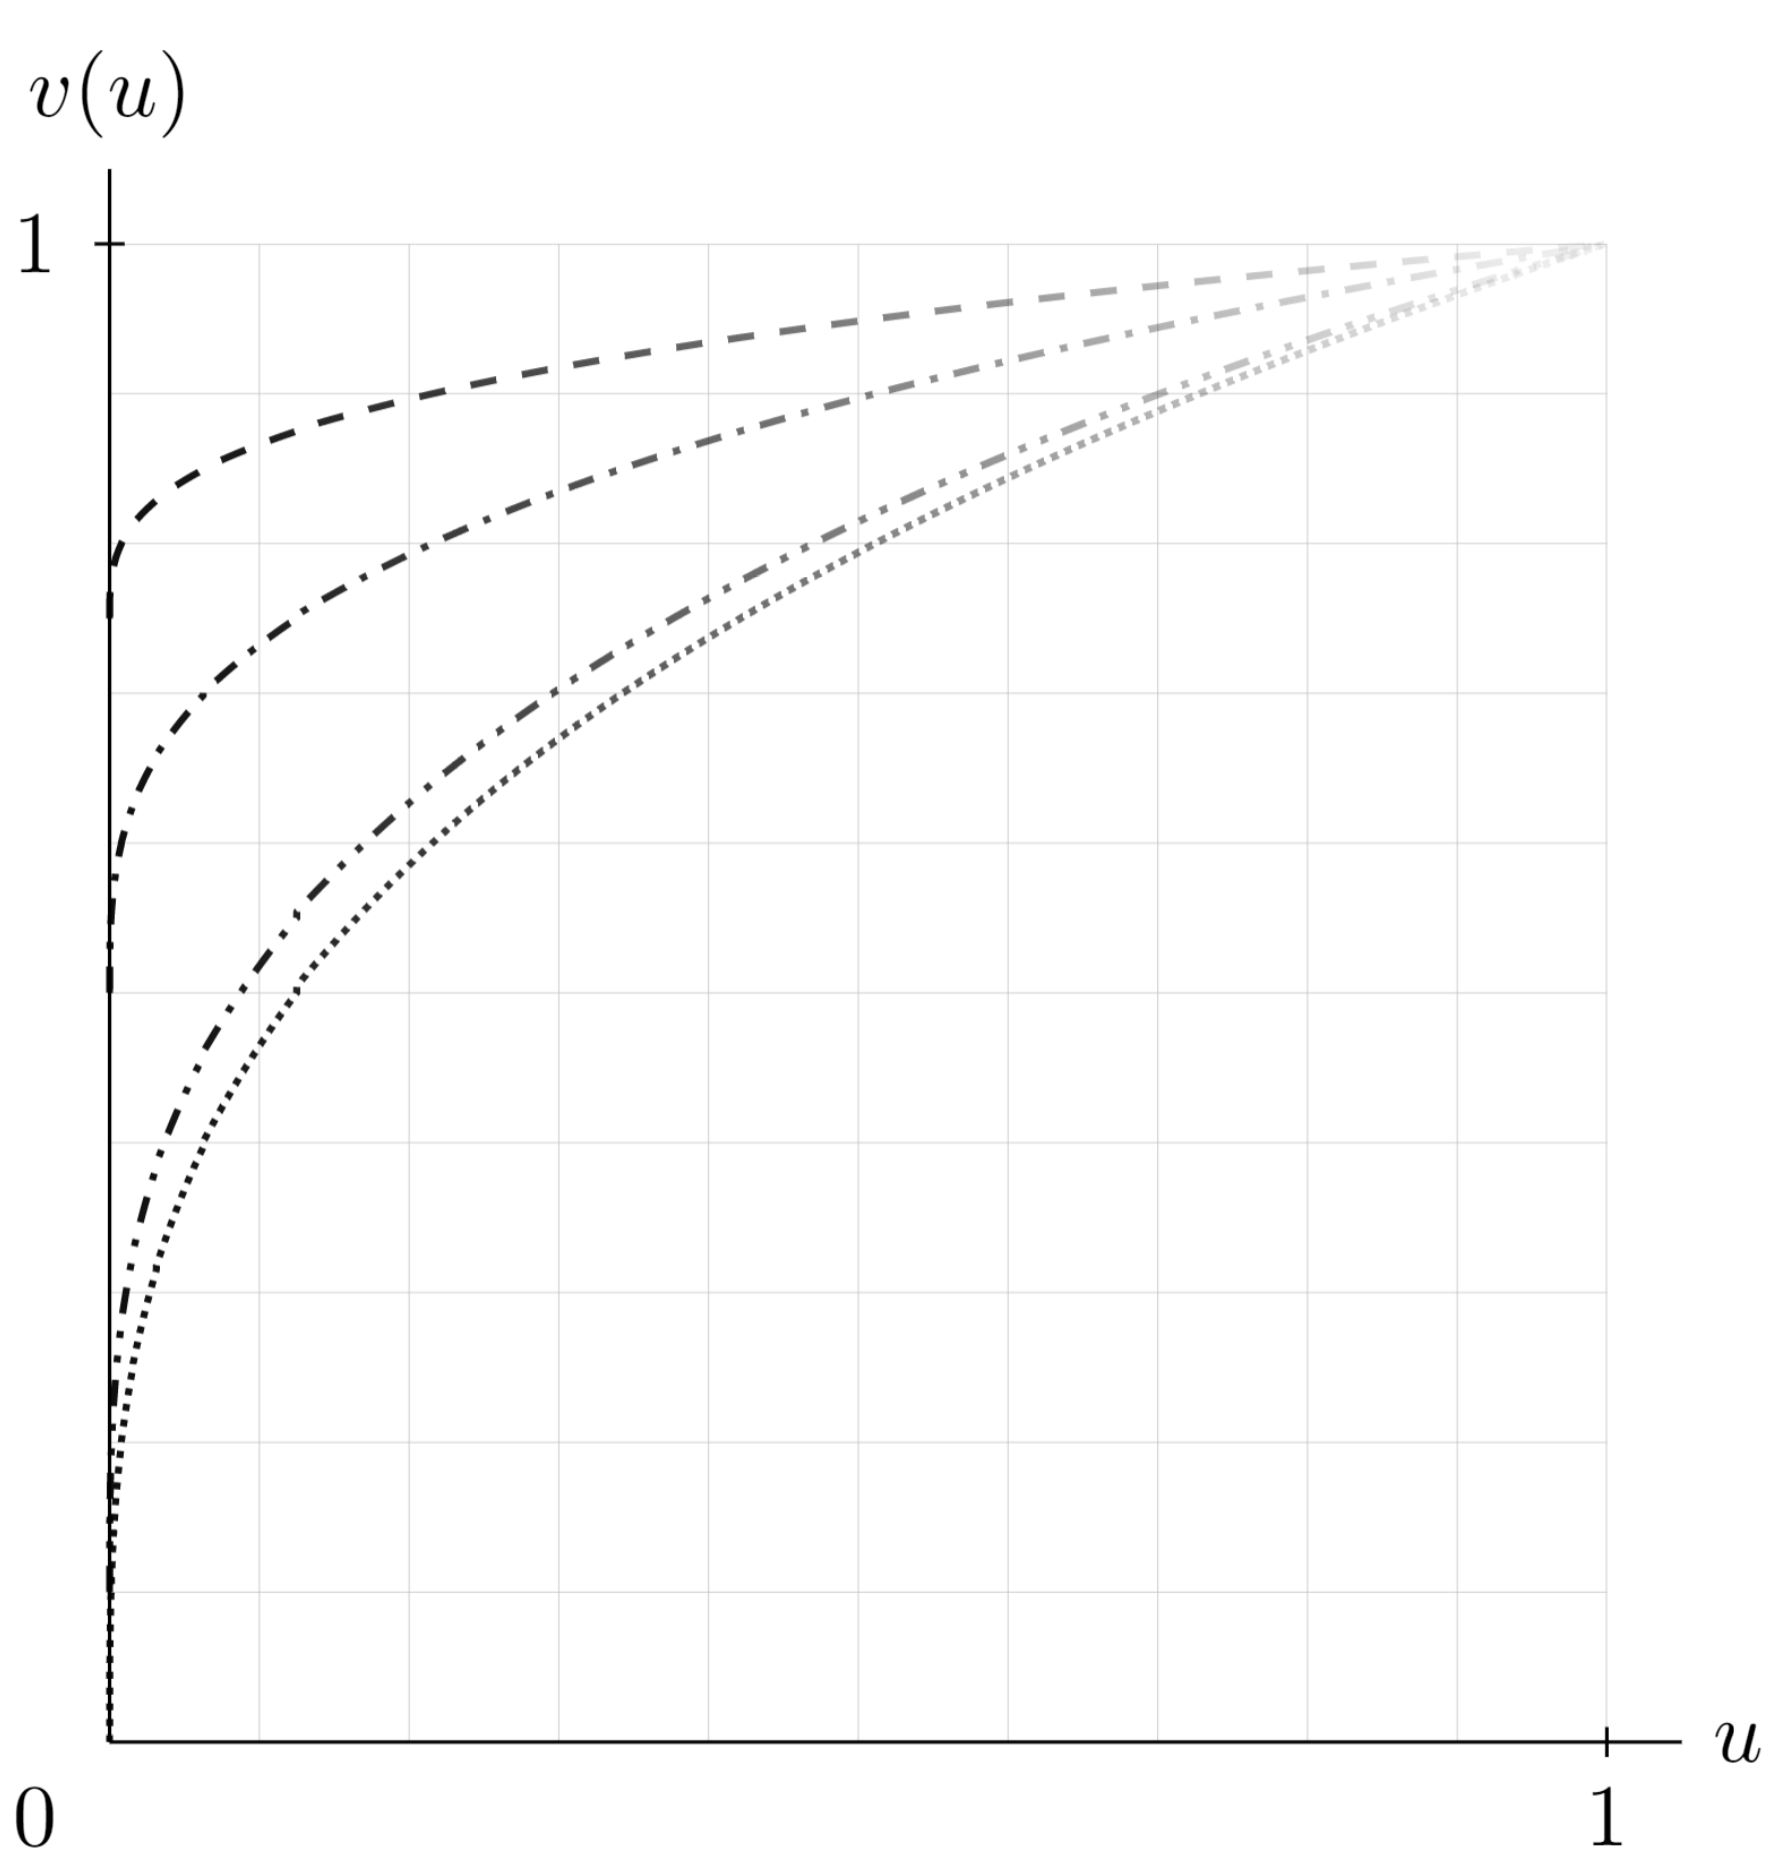
\includegraphics[width=\textwidth]{fig_skilltech}
        \caption{Technology of skill enhancement.}
    \end{subfigure}
    \hfill
    \begin{subfigure}[t]{0.45\textwidth}
        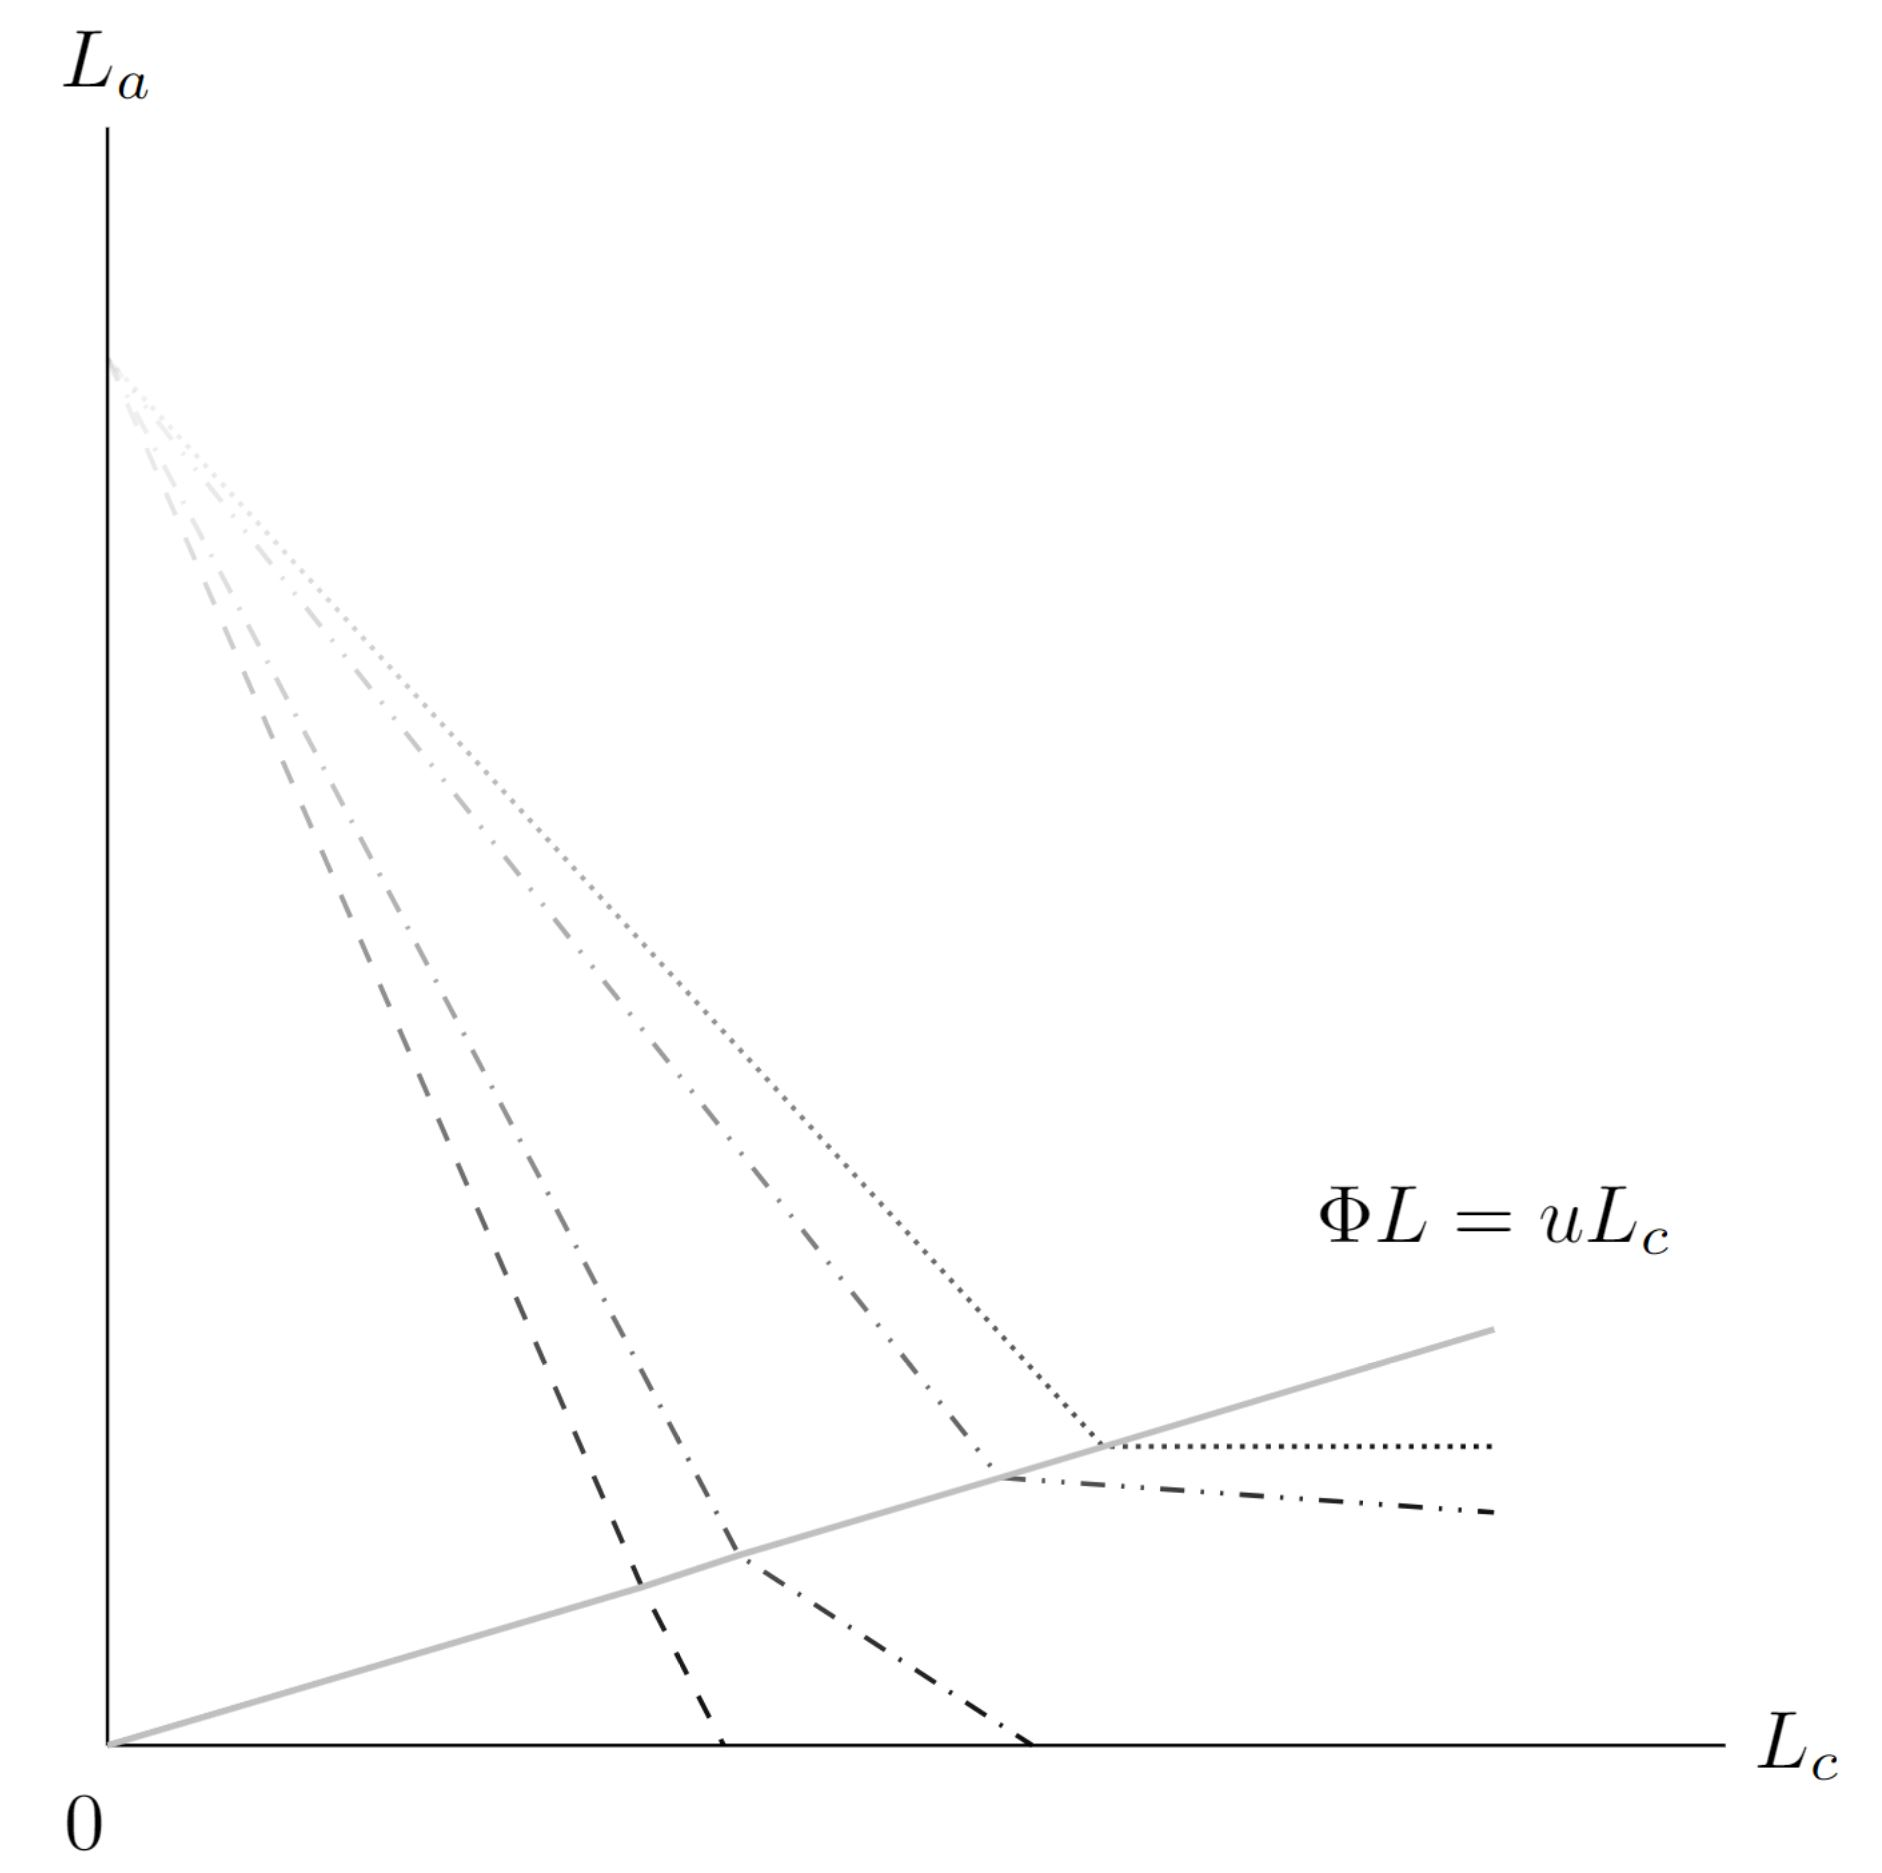
\includegraphics[width=\textwidth]{fig_isoquants}
        \caption{Effective labour isoquants.}
    \end{subfigure}
    \caption*{\footnotesize{\textit{Note:} (a) The figure graphs four versions of the function $v(u)=v_0+(\overline{v}-v_0)u^{\frac{1}{3}}$ for different values of raw skill $v_0$. The dotted curve corresponds to $v_0=0$ and the curves above it to $v_0=0.1$, to $v_0=0.5$, and to $v_0=0.75$ respectively. (b) The dotted isoquant corresponds to $v_0=0$, whereas the isoquants to its left correspond to $v_0=0.1$, to $v_0=0.5$, and to $v_0=0.75$ respectively. The upward sloping line in gray, which connects the isoquant kinks, is defined by its slope, the intensity of supervision $u$. \textit{Source:}  author's own compilations.}}
    \label{fig:model}
\end{figure}


The adult-labour equivalents of any given combinations of adult and child labour, considering the complementary of supervision in addition to the substitution between $L_a$ and $L_c$, can be captured by the household's effective labour supply:

\begin{equation}
\label{eq:labsup}
    L_{\mathcal{I}} =
        \begin{cases}
            L_A - s u L_C + s v(u) L_C + (1-s) v_0 L_C & \text{if} \quad s u L_C < L_A \\
            v(u) \frac{L_A}{u} + v_0 \left(L_c - \frac{L_A}{u}\right) \quad & \text {if} \quad s u L_C = L_A
        \end{cases}
        .
\end{equation}

This specification allows for the household decision maker to choose flexibly not only the levels of adult and child labour supply, but also the fraction of children to work with and without supervision, as well as the intensity of such supervision; all this in view of optimising the household's welfare. Setting $v_0=0$, $s=1$, $u<1$ and $v(u)=1 \quad \forall u$, equation \ref{eq:labsup} simplifies to the labour supply function in \citet{Bar2009}. Panel (b) of figure \ref{fig:model} plots combinations of child and adult labour, using the same values for $v_0$ as in Panel (a). The dotted curve on top corresponds to the Bar and Basu perspective that unsupervised child labour must be entirely unproductive (i.e. $v_0=0$).\footnote{For all functions graphed in figure \ref{fig:model}, it is assumed that $u=0.1$ and $s=1$.} Note that along each of the piece-wise linear functions in panel (b), the effective labour input $L$ stays the same, indicating that, holding other inputs constant, they are isoquants in the farm production problem to which I turn next 

\paragraph{Agricultural production:}
Agricultural products are produced using labour $L$ and quasi-fixed land and capital $K$. The quantity produced is given by $Q=f(L,\theta,K)$, where $\theta \in\mathbb{R}_+$ is a weather-dependent productivity factor and $f(\cdot)$ is a continuous and twice differentiable production function, for which the following four inequalities hold:

$$\frac{\partial f}{\partial L}>0 \quad \frac{\partial f}{\partial \theta}>0 \quad \frac{\partial^2 f}{\partial L^2}<0 \quad \frac{\partial^2 f}{\partial L \partial \theta}>0.$$

\paragraph{Household problem:}

Household $\mathcal{I}$ is a price-taker in all markets and maximises utility in every period subject to a full income constraint $Y$, which includes agricultural profits and the value of the household's time endowment $I$. Formally,
\begin{align}
\label{eq:UMP}
    &\max_{L_A, L_C,X_1, X_2, X_3, X_4} U(\mathbf{X})\\ 
\label{eq:budget_constraint}
    s.t.\quad& p_1 X_1 + p_2 X_2 + p_3 X_3 +p_4 X_4 = Y=p_3 f(L,\theta,K)-p_2L+p_2I
\end{align}
where $p_1$, $p_2$, $p_3$ and $p_4$ are the prices for non-agricultural products and services, child labour, adult labour, and agricultural products. Plugging equations (\ref{eq:UF}) and (\ref{eq:labsup}) into (\ref{eq:UMP}) and (\ref{eq:budget_constraint}) above, and solving the production side of this model, it can be shown that




%%%%%%%%%%%%%%%%%%%%%%%%%%%%%%%%%%%%%%%%%%%%%
%%%%%%%%%%%%%%%%%%%%%%%%%%%%%%%%%%%%%%%%%%%%%
%%%%%%%%%%%%%%%%%%%%%%%%%%%%%%%%%%%%%%%%%%%%%

\subsection{Hypotheses}

\section{Empirical Analysis}
\label{sec:empirical_analysis}

\subsection{Case Selection}
\label{sub:case_selection}

Nigeria is the most populous and the sixth-most densely populated country in Africa\footnote{With a population of 200 million, Nigeria is also the sixth-most populous country in the world.}, and its 2020 nominal GDP of USD $450$ billion makes it the biggest economy on the continent \citep{WorldBank2021}.\footnote{In terms of purchasing power parity, only Egypt narrowly outperforms Nigeria.} About half of the population live in urban areas, particularly the large metropolitan areas in the South and Southwest towards the country's coast on the Gulf of Guinea. Moving North, the population density decreases gradually, giving way to wide savannahs and steppes which are characterised predominantly by agriculture.

Nigeria exhibits some characteristics which make it a particularly well-suited case study in the context of this paper. First, while exact estimates are hard to come by, it is generally acknowledged that child labour is rampant. The \citet{USDepartmentofLabor2021} estimates that 13 million children work on a regular basis. In May 2019, the ILO's Country Office Director stated publicly that at least 43 percent of Nigerian children - 15 million - were trapped in forced, largely unpaid labour \citep{ILO2019}. This is double the SSA average, which itself is the highest regional average in the world. While child work is also common in other sectors, such as domestic servitude or gold mining, the vast majority of working children are employed on their families' farms.

Second, Nigeria exhibits high levels of (rural) poverty and socio-economic inequality. Although it is one of the fastest-growing countries in the world, almost half of its population still grapples with extreme poverty. With a Gini index of 35, income inequality lies close to the SSA average. This shows a highly uneven distribution of wealth between many poor and very few rich households. According to the most recent national report, 40 percent of the total population, or almost 83 million people, lived below the country's poverty line of 137,439 Naira (USD 381.75) per person per year. While most wealth is located in the big metropolitan areas such as Lagos, Ibadan, and Abuja, poverty is both more prevalent and deeper in rural areas, where the headcount is above 50 percent and the poverty gap amounts to 17.4 percent of the poverty line on average in contrast to a mere four percent observed in urban areas \citep{NBS2020}.

The simultaneous concentration of (extreme) poverty and rampant child labour in rural areas closely resembles two key assumptions of the model derived in section \ref{sec:model}: the luxury axiom, operationalised by the subsistence terms in the Stone-Geary utility function, operationalises the assumption that poverty is the principle driver of child labour. The agricultural focus of most households' economic activity further suggests a large enough subpopulation of specifically agricultural child labour to properly estimate the effects of climate change on this group. Taken together, these facts make Nigeria a highly relevant and suitable context for testing the model's hypotheses about agricultural child labour.

\subsection{Data sources and processing}
\label{sub:data_sources}
Analysing the prevalence of child labour as a function of climate change must involve at least two types of data: weather observations and individual-level work data for children. In order to enrich this analysis and control for possible confounders, other individual and household characteristics should be added. To obtain a clearer image of the agricultural production process, community and household data on agricultural variables and market structure are also required. A last and absolutely vital requirement is, of course, that all these data are geo-coded in accordance with a coordinate reference system (usually degrees of latitude and longitude).

This study relies on two data sources to meet these requirements. First, the individual, household, and community variables are provided by the Nigeria General Household Survey (GHS), which is part of the World Bank's Living Standards Measurement Surveys (LSMS) programme and is conducted by Nigeria's National Bureau of Statistics in collaboration with Nigeria's Federal Ministry of Agriculture and Rural Development, the National Food Reserve Agency, the Bill and Melinda Gates Foundation and the World Bank. GHS is an ongoing long-term project to create a growing panel of agricultural and household data in such a way as to allow the study of agriculture’s role in household welfare over time. It collects information on household agricultural activities along with other information on the households like human capital, other economic activities, and access to services and resources.

The GHS-Panel lends itself extremely well to this paper's research question thanks to its succinctly agricultural focus. To date, the survey instrument has produced four waves (2010-2011, 2012-2013, 2015-2016, 2018-2019), the first three of which are used in this analysis. Each wave of the GHS-Panel is a cross-section of approximately 22,000 individuals in approximately 5,000 households which are representative of the Nigerian population at large. The decision to omit the most recent wave in this analysis was taken due to what seems to be non-random attrition of households after wave 3, concentrated in the rural areas that are so central to this paper.

Each GHS wave consists of two visits, one at the end of the planting season, between September and November, and the other at the end of the harvest, February thru April of the following year. The three waves thus record observations at six distinct points in time and the final panel has six rather than three layers.

The most relevant parts of the GHS panel are the individuals' labour information (e.g., hours worked, wages earned, sectoral information, and time spent on household chores), agricultural plot and production information by household, as well as the more general socio-economic standing of the households and their individual members. This includes education, which is of particular interest as it may compete with child labour for children's time allocation. Apart from its agricultural focus, what sets the GHS apart is the decision by its creators to include approximate spatial coordinates of the enumeration areas (EA) where the households are located.\footnote{EAs are the smallest geographical partition present in the GHS, approximately equivalent to a community or a cluster of villages. Other, higher order units are equivalent to Nigeria's administrative divisions of Legislative Government Areas (LGA), provinces, and regions.} This allows users to spatialise the dataset and combine it with other data sources according to the coordinates attached.

\begin{figure}[t!]
    \centering
    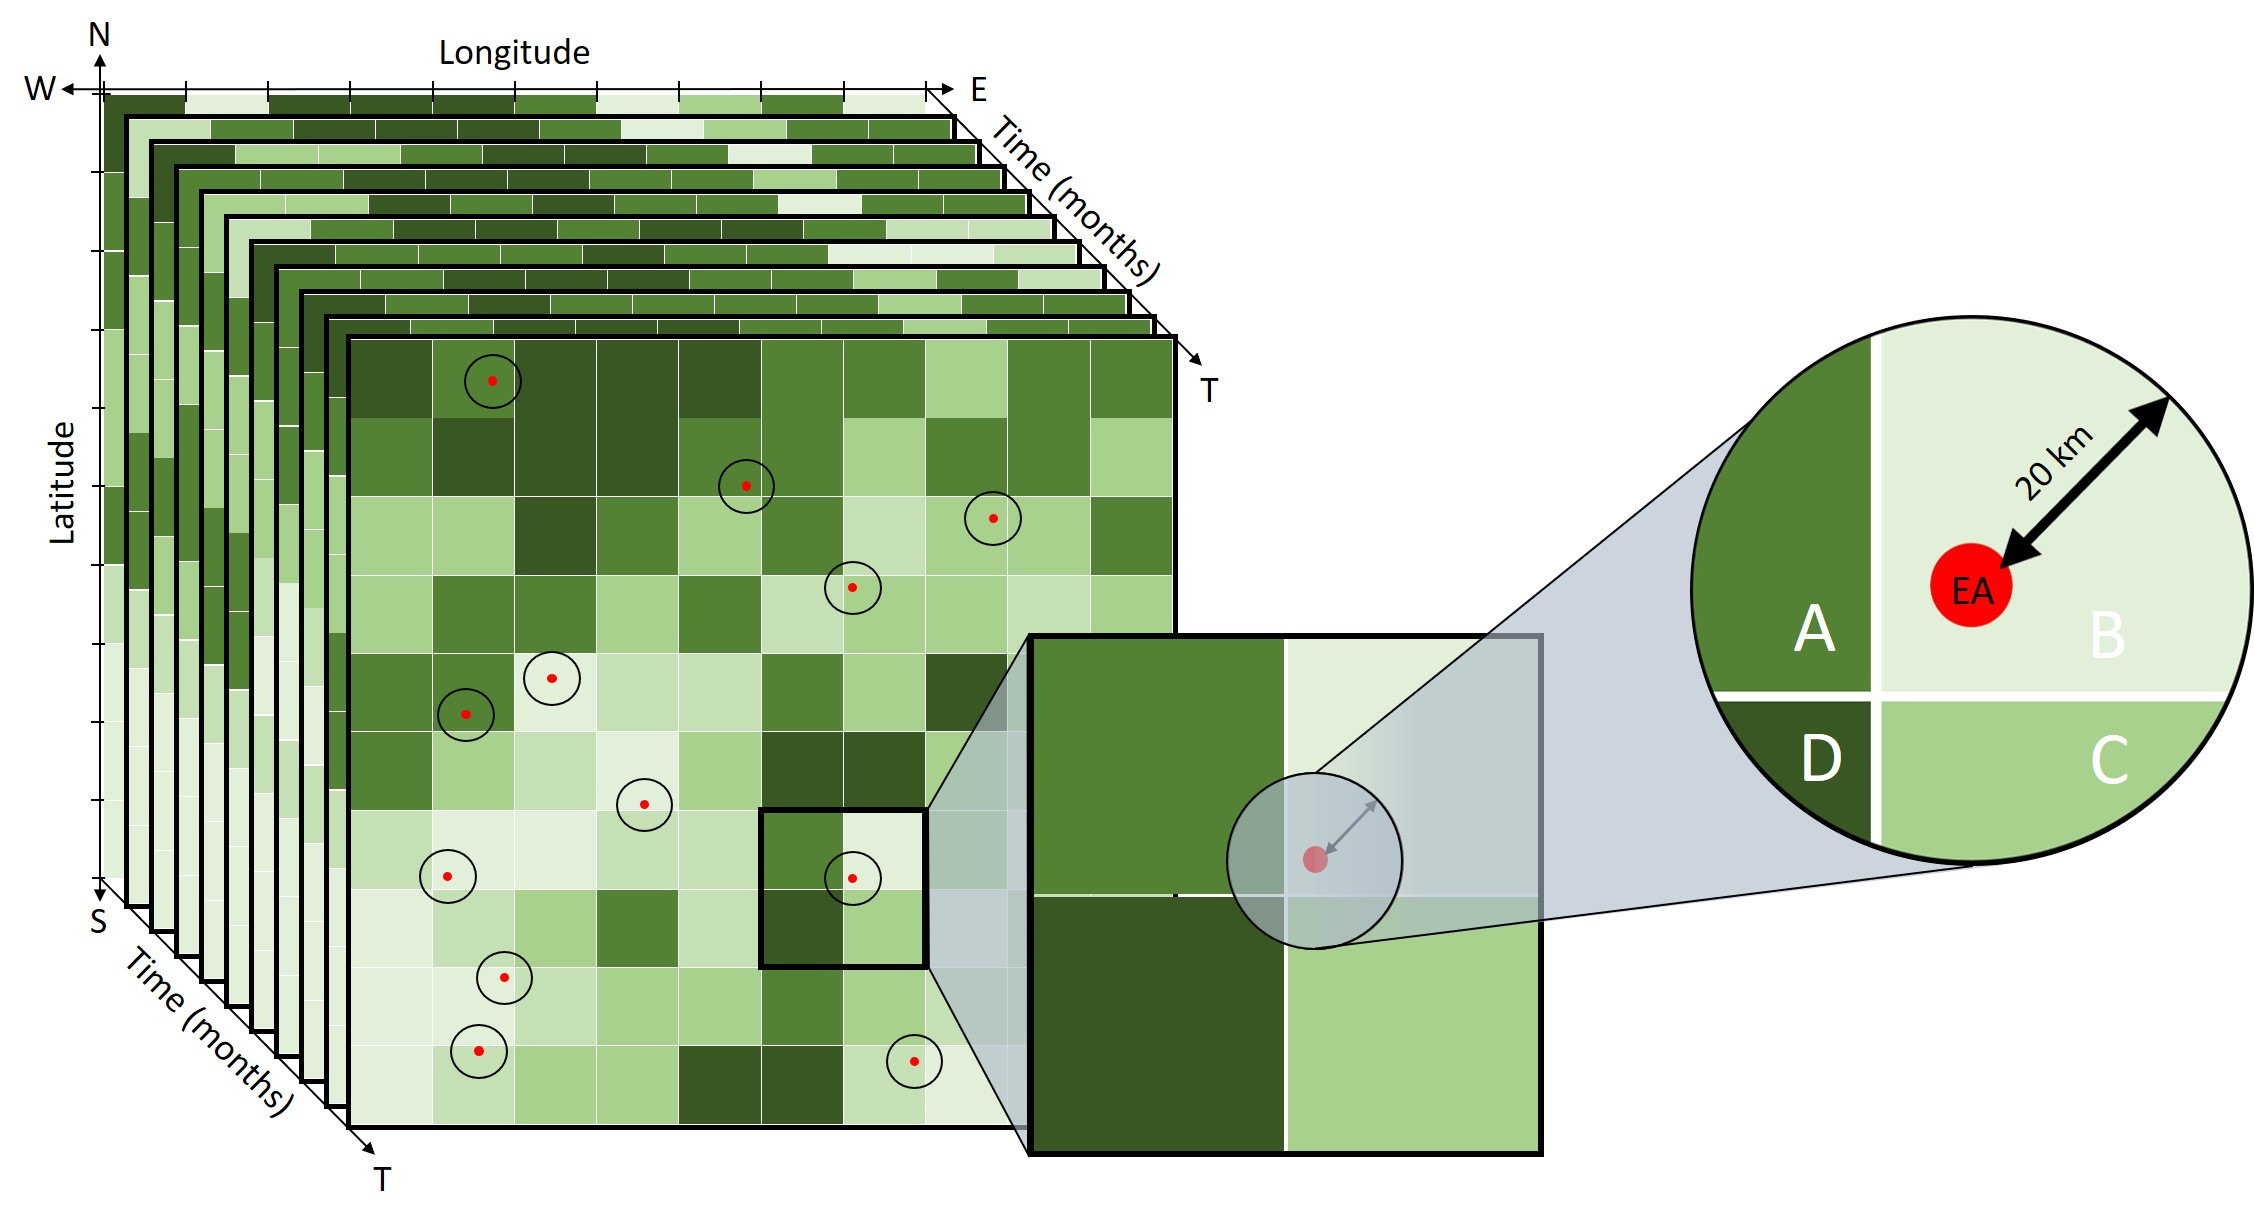
\includegraphics[scale=0.33]{../outputs/buffer.JPG}
    \caption{Smoothing climate variables using a circular buffer}
    \caption*{\footnotesize{\textit{Note:} Time series of climate variables take the form of three dimensional ``stacks'' of coordinate grids, one for each timepoint. Each of these grids is composed of cells. Every cell, in turn, holds the measured value of the variable within its spatial limits at the grid's time point. The three dimensional grid stack on the left has the following axes: latitude from North (N) to South (S), longitude from West (W) to East(E), and discrete time in monthly intervals (T). Every grid's cells are coloured in shades of green that indicate the value of the climate variable on a continuous scale (e.g. monthly mean temperature in degrees celsius). The red dots represent the EA locations from the spatialised GHS data. Around every EA centroid, a circular buffer with radius $r=20$ kilometres is drawn. The exact value at the EA's location is then imputed by taking the weighted average of the cell segments (in order of size) B, A, C, and D that fall within the buffer, weighted by their respective surface areas. \textit{Source:} Author's own compilation.}}
    \label{fig:buffer}
\end{figure}

In this case study, I spatialise the dataset and combine it with climate data. Version 4.05 of CRU TS (Climatic Research Unit gridded Time Series) is a widely used global climate dataset. It is derived by the interpolation of monthly climate anomalies from extensive networks of weather station observations.\footnote{For detail on how CRU TS was constructed, see the accompanying publication \citep{harris2020}.} CRU TS 4.05 includes ten timeseries of geophysical variables that jointly depict the development of the world's at a monthly interval. This data, which is available from January 1901 to December 2020, is laid out on a 0.5° latitude by 0.5° longitude grid (approximately 50 kilometres by 50 kilometres cells) across all major land masses (other than Antarctica). This high resolution allows capturing a great part of cross-community climate variation between EAs.

For every EA in the GHS dataset, I compute the location-specific timeseries for every climate variable in CRU TS 4.05. To smoothen transitionary differences between climate cells, every EA's climate variables are obtained by taking a weighted average of all the cells which fall within a circular buffer of $r$ kilometres around the EA's centroid coordinates. This computation increases the variability of the climate data further, mirroring the resolution of EAs by averaging over two or more cells. Therefore, depending on the length of $r$, climate variables at the EA coordinates is a composition of one or more cell values. Whenever the buffer crosses into adjacent cells, the EA is assigned the area-weighted arithmetic mean of its own cell and the adjacent ones within the $r$ kilometre radius.\footnote{For the computational implementation, see the \texttt{buffer} option of the \texttt{extract} command from the \texttt{R}-library \href{https://cran.r-project.org/web/packages/raster}{\texttt{raster}} \citep{hijmans2020} and its successor \href{https://cran.r-project.org/web/packages/terra}{\texttt{terra}} \citep{hijmans2021}.} Figure \ref{fig:buffer} is a schematic representation of this procedure. As there are no missing values in CRU TS, ten full monthly time series (one per variable) can be created for 1999-2020.

\subsection{Variables}
\label{sub:variables}

This section briefly describes the main variables used in the analysis and how they were constructed.

\subsubsection{GHS variables}
\label{subsub:ghsvars}
The survey recorded the ``hours worked last week in a job'', as well as the ``minutes spent on chores yesterday''. In order to streamline the time-frame of these two variables, the hours worked in a job are divided by seven and the minutes spent on chores are divided by sixty. Adding up the two results for every individual gives their daily work hours including chores.\footnote{Note that this often yields non-integer values due to the conversion of the chore variables from minutes to hours. Moreover, this construction relies on the assumptions that (i) last week's workload is representative for the overall workload, and (ii) that yesterday's chore minutes are representative of every day's time spent on chores.} Lastly, I filter the variable by age and set it to missing for individuals aged 18 or above. The final result is an approximate measure of daily hours spent in child labour including chores.\footnote{Alternative measures can be obtained, for instance by omitting the chores component or by filtering out observations outside the agricultural sector. All these alternative measures turn out to be virtually equivalent with correlations among them and the original variable ranging between $0.92$ and $1$. Since the additional constraints do, however, cost observations I proceed with the initially proposed variable.}

Other variables which are taken more or less unaltered from the GHS-panel\footnote{In some cases, they were recoded to subsume many categories into one or to facilitate interpretation of results.} are years of schooling, highest achieved educational level (by terms), household income, household size, age-order among the household's children, sex, sex of the household head, employment details of the household's adults, size and quality of the agricultural land owned by the household, as well as amenities and services enjoyed by its members. The latter include the distance to important community locations like roads, markets, hospitals, or village centres, as well as the presence and quality of water supply, sanitation, roofing, and the overall quality of shelter.

To assess the welfare of a given household, a multidimensional poverty index (MPI) is constructed, closely following the approach spearheaded by \citet{alkire2011} and most recently used applied globally in \citet{alkire2020}. I retain the same dimensions, indicators, and relative weights used in \citet{alkire2018, alkire2020}, subject to data availability in the GHS. Each of the indicators used is related explicitly to one or more of the SDGs.\footnote{For the parallel joint publication by OPHI and UNDP see \href{http://hdr.undp.org/sites/default/files/2020_mpi_report_en.pdf}{here}. }Multidimensional indices are particularly attractive because they can be disaggregated, as discussed in \citet{bourguignon2003, foster1984}, in addition to fulfilling the properties usually required by poverty metrics \citep[see][]{Sen1976}.\footnote{For a critical review of the MPI literature, see \citet{ravallion2011}.}

The health dimension is comprised of three indicators. Nutrition, which is related to SDG 2 ``Zero Hunger'', codes a household as deprived if there was a situation in the last 12 months when there was not enough food to feed the household members. Child mortality is measured by the number of male and female children, born to women between 12 and 49, who died in the household. If this number is, on average across the household's eligible females, 1 or greater the household codes as deprived. Child mortality relates directly to SDG 3 ``Health and Wellbeing". Both measures are equally weighted 1/6 each so that health accounts for a third of the MPI. 

The education dimension also consists of two indicators. Years of schooling codes a household as deprived if no eligible household member has completed six years of schooling. Second, a household is deprived in terms of school attendance if any of its school-aged children is not attending school at the age-appropriate level up to class eight. Both education indicators are clearly related to SDG 4 ``Quality Education"Again, each of the education indicators is weighted 1/6, giving education a total weight of 1/3.

The last dimension of poverty is living standards, measured by six variables which are each weighted 1/18. A household is deprived in cooking fuel, if it cooks using solid fuel such as dung, agricultural crop, shrubs, wood, charcoal, or coal. In terms of electricity, a household is deprived if it has no electricity in the home. Both cooking fuel and electricity are central to SDG 7 ``Affordable and Clean Energy''. Sanitation deprivation occurs if a household has no or only an unimproved sanitation facility, or if it has an improved facility but shared with another household. A household is coded as deprived of drinking water if its source of drinking water is not safe for human consumption or if safe drinking water is 30 minutes or longer away by foot (round trip). Both sanitation and drinking water are basic needs acknowledged in SDG 6 "Clean Water and Sanitation".

In relation to SDG 11 ``Sustainable Cities and Communities'', a household is deprived in housing if it has inadequate housing materials in any of the three components floor, roof, or walls. Lastly, a household is considered asset deprived if it does not own more than five of the these: sofa, chairs, table, mattress, bed, mat, sewing machine, gas cooker, electric stove, gas stove, kerosene stove, fridge, freezer, air conditioner, washing machine, electric clothes dryer, bicycle, motorbike, car or other vehicle, generator, fan, radio, cassette recorder, Hi-Fi sound system, microwave oven, iron, television set, computer, DVD player, satellite dish, and musical instrument. The indicator of asset deprivation is related to SDG 1 ``No Poverty''.

\subsubsection{Climate variables}
\label{subsub:climatevars}

As mentioned above, CRU TS includes timeseries of ten different geophysical variables. They can be further categorised as primary, secondary, and derived variables. Primary variables are those that are directly measured at ground station level and have no synthetic component. They are mean temperature over two months (TMP), diurnal temperature range  over two months (DTR), and the precipitation rate (PRE).

Secondary Secondary variables differ from primary variables in that they have fewer direct observations available. The synthetic estimates are estimated using empirical relationships with the primary variables. Vapour pressure (VAP) is generated from TMP, and DTR as described in \citet{harris2020}. The count of wet days (WET) is defined as the number of days in a month on which PRE $\geq0.1$ millimetres - a metric used in diverse areas including evaluation of satellite observations and of potential evapotranspiration equations. It is compiled using the same interpolation algorithm as in \citet{harris2014}. Synthetic cloud cover observations (CLD) are computed from DTR as in \citet{harris2014}, using station-based values. DTR is the percentage of cloud coverage averaged over the month.

Derived variables are entirely synthetic as their values are imputed from the observed values using empirically validated formulae. Minimum and Maximum temperature over two months (TMN and TMX) are derived arithmetically from TMP and DTR as described in \citet{harris2014}. Both are useful metrics, for instance for monitoring droughts, agronomic production and river basin vegetation. Freezing days per month (FRS) is the number of days in a month that record TMN $\leq 0$ degree Celsius. It is derived from TMN using an empirically determined function and is commonly used in dendroclimatology and health. Lastly, potential evapotranspiration (PET) is calculated from TMP, VAP, and CLD using the Penman-Monteith formula \citep{allen1998}, the United Nations Food and Agriculture Organization's (FAO) standard method for modelling evapotranspiration, as explained in \citet[][pp. 1071 - 1072]{ekstrom2007}. PET is defined as the amount of evaporation from the ground into the atmosphere that would occur if a sufficient water source were available. It is an important variable with regards to agriculture as it directly affects plant growth. If PET exceeds PRE, a place is considered dryland.

Table \ref{tab:cruvars} shows the variables of CRU TS, their units and their correlation decay distances (CDDs). A variable's CDD is defined as the distance where the correlation between one station and all other stations decays below $1/e$. The search radius for the selection of stations for the interpolation in CRU TS is set equal to the CDD as this optimises accuracy \citet{harris2020}. In other words, CDD is the distance between a station and a grid cell beyond which a station's raw observations are not useful for interpolating the climate variable at the cell. Generally speaking, precipitation has a rather low CDD as it is highly spatially concentrated, whereas temperature and vapour pressure usually vary over greater distances.

\begin{table}[t!]
    \singlespacing
    \centering
    \caption{CRU TS variables, showing codes, units, correlation decay distances (CDDs).}
    \caption*{\footnotesize{\textit{Notes:} A wet day is one receiving $\geq 0.1$ mm precipitation. Minimum and maximum temperatures are the monthly means of the individual daily minimum and maximum temperatures; they are not the overall minimum or maximum temperature recorded each month. \textit{Source:} adapted from \citet{harris2020}.}}
    \begin{tabular}{|p{6cm}|p{1cm}|p{3cm}|p{2cm}| }
    \hline
    \raggedright\textbf{Variables} & \textbf{Code} & \textbf{Units} & \textbf{CDD(km)} \\
    \hline    
    \textbf{Primary} & \ \ & \ \ & \ \ \\
    \quad Mean 2m temperature & TMP & degrees Celsius & 1200\\
    \quad Diurnal 2m temperature range & DTR & degrees Celsius & 750 \\
    \quad Precipitation rate & PRE & mm/month & 450 \\
    \textbf{Secondary} & \ \ & \ \ & \ \ \\
    \quad Vapour pressure & VAP & hPA & 1000 \\
    \quad Wet days & WET & days/month & 450 \\
    \quad Cloud cover & CLD & percentage & 600 \\
    \textbf{Derived} & \ \ & \ \ & \ \ \\
    \quad Frost days &FRS& days/month & 750 \\
    \quad Minimum 2m temperature &TMN& degrees Celsius & 1200 \\
    \quad Maximum 2m temperature &TMX& degrees Celsius & 1200 \\
    \quad Potential evapotranspiration &PET& mm/day & n/a \\
    \hline
    \end{tabular}
    \label{tab:cruvars}
\end{table}

Since the economic model presented in section \ref{sec:model} assumes that climate effects enter the household's problem through its impact on agricultural production, it is quintessential to link the household data with the climate variables measured during the relevant growing season rather than over the entire year.



\begin{sidewaysfigure}
\centering
    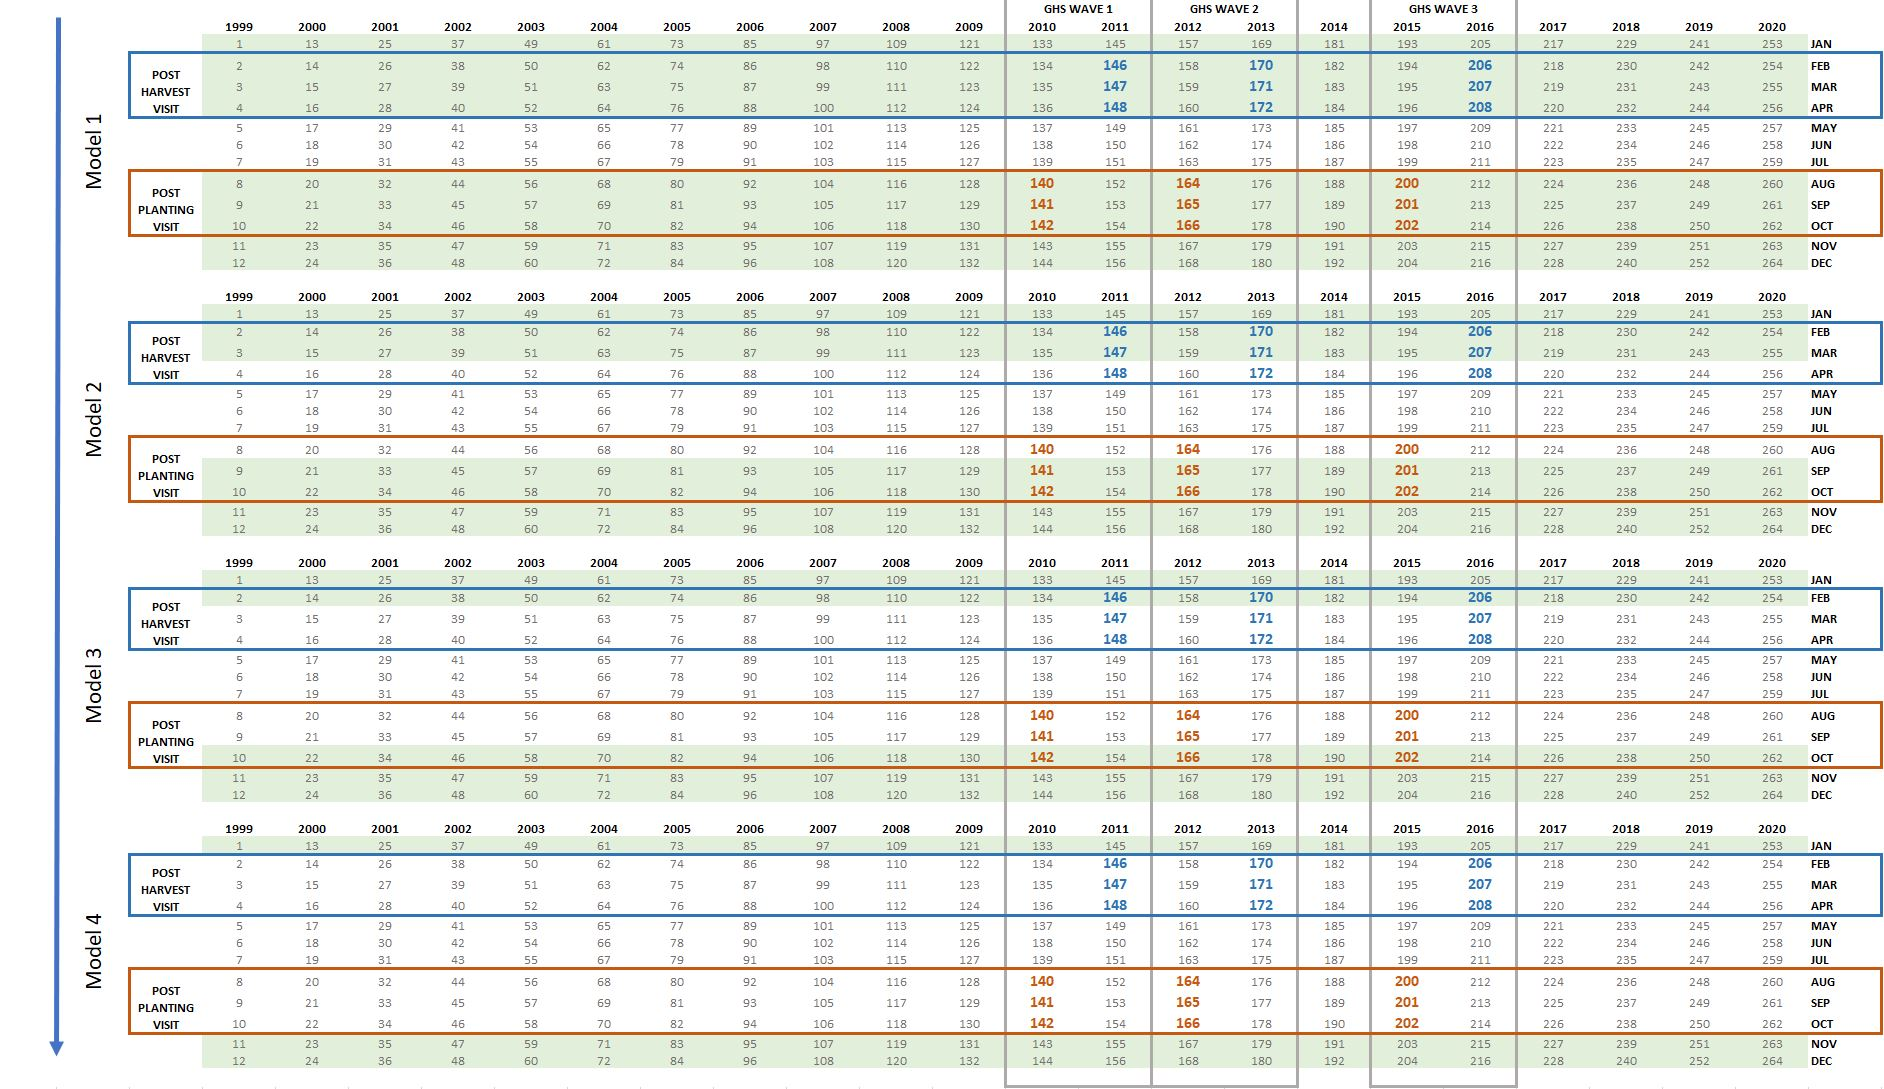
\includegraphics[scale=0.58]{../outputs/timing.JPG}
    \caption{Approximate delimitation of the growing season.}
    \caption*{\footnotesize{\textit{Note:} Four models of increasing data scarcity. Numbers denote monthly ID from 1 (January 1999) to 264 (December 2020). The bold coloured numbers denote time spans for which there is household data available from the GHS waves 1-3, brown being post planting and blue being post-harvest visits. Lastly, the growing season is denoted by green cells. The most data-abundant delimitation includes climate data from the months when visits happen. From this model 1, further variations exclude months until the growing season is delimited to months after the post-planting and before the post-harvest visits entirely.}}
\label{fig:buffer}
\end{sidewaysfigure}

\subsection{Econometric strategy:}
\label{sub:econometric_strategy}



\section{Findings}
\label{sec:findings}

%\section{Simulation}
\label{sec:simulation}

%\subsection{Climate model input}
\label{sec:climate_model_input}

%\subsection{Predictions}
\label{sec:predictions}

%\section{Discussion}
\label{sec:discussion}

\section{Conclusion}
\label{sec:conclusion}



\newpage
\small
%\nocite{*}
\bibliographystyle{apalike}
\bibliography{References}

\newpage
\appendix

\end{document}